\PassOptionsToPackage{unicode=true}{hyperref} % options for packages loaded elsewhere
\PassOptionsToPackage{hyphens}{url}
%
\documentclass[]{article}
\usepackage{lmodern}
\usepackage{amssymb,amsmath}
\usepackage{ifxetex,ifluatex}
\usepackage{fixltx2e} % provides \textsubscript
\ifnum 0\ifxetex 1\fi\ifluatex 1\fi=0 % if pdftex
  \usepackage[T1]{fontenc}
  \usepackage[utf8]{inputenc}
  \usepackage{textcomp} % provides euro and other symbols
\else % if luatex or xelatex
  \usepackage{unicode-math}
  \defaultfontfeatures{Ligatures=TeX,Scale=MatchLowercase}
\fi
% use upquote if available, for straight quotes in verbatim environments
\IfFileExists{upquote.sty}{\usepackage{upquote}}{}
% use microtype if available
\IfFileExists{microtype.sty}{%
\usepackage[]{microtype}
\UseMicrotypeSet[protrusion]{basicmath} % disable protrusion for tt fonts
}{}
\IfFileExists{parskip.sty}{%
\usepackage{parskip}
}{% else
\setlength{\parindent}{0pt}
\setlength{\parskip}{6pt plus 2pt minus 1pt}
}
\usepackage{hyperref}
\hypersetup{
            pdftitle={graphsim: An R package for simulating gene expression data from graph structures of biological pathways},
            pdfborder={0 0 0},
            breaklinks=true}
\urlstyle{same}  % don't use monospace font for urls
\usepackage[margin=1in]{geometry}
\usepackage{color}
\usepackage{fancyvrb}
\newcommand{\VerbBar}{|}
\newcommand{\VERB}{\Verb[commandchars=\\\{\}]}
\DefineVerbatimEnvironment{Highlighting}{Verbatim}{commandchars=\\\{\}}
% Add ',fontsize=\small' for more characters per line
\usepackage{framed}
\definecolor{shadecolor}{RGB}{248,248,248}
\newenvironment{Shaded}{\begin{snugshade}}{\end{snugshade}}
\newcommand{\AlertTok}[1]{\textcolor[rgb]{0.94,0.16,0.16}{#1}}
\newcommand{\AnnotationTok}[1]{\textcolor[rgb]{0.56,0.35,0.01}{\textbf{\textit{#1}}}}
\newcommand{\AttributeTok}[1]{\textcolor[rgb]{0.77,0.63,0.00}{#1}}
\newcommand{\BaseNTok}[1]{\textcolor[rgb]{0.00,0.00,0.81}{#1}}
\newcommand{\BuiltInTok}[1]{#1}
\newcommand{\CharTok}[1]{\textcolor[rgb]{0.31,0.60,0.02}{#1}}
\newcommand{\CommentTok}[1]{\textcolor[rgb]{0.56,0.35,0.01}{\textit{#1}}}
\newcommand{\CommentVarTok}[1]{\textcolor[rgb]{0.56,0.35,0.01}{\textbf{\textit{#1}}}}
\newcommand{\ConstantTok}[1]{\textcolor[rgb]{0.00,0.00,0.00}{#1}}
\newcommand{\ControlFlowTok}[1]{\textcolor[rgb]{0.13,0.29,0.53}{\textbf{#1}}}
\newcommand{\DataTypeTok}[1]{\textcolor[rgb]{0.13,0.29,0.53}{#1}}
\newcommand{\DecValTok}[1]{\textcolor[rgb]{0.00,0.00,0.81}{#1}}
\newcommand{\DocumentationTok}[1]{\textcolor[rgb]{0.56,0.35,0.01}{\textbf{\textit{#1}}}}
\newcommand{\ErrorTok}[1]{\textcolor[rgb]{0.64,0.00,0.00}{\textbf{#1}}}
\newcommand{\ExtensionTok}[1]{#1}
\newcommand{\FloatTok}[1]{\textcolor[rgb]{0.00,0.00,0.81}{#1}}
\newcommand{\FunctionTok}[1]{\textcolor[rgb]{0.00,0.00,0.00}{#1}}
\newcommand{\ImportTok}[1]{#1}
\newcommand{\InformationTok}[1]{\textcolor[rgb]{0.56,0.35,0.01}{\textbf{\textit{#1}}}}
\newcommand{\KeywordTok}[1]{\textcolor[rgb]{0.13,0.29,0.53}{\textbf{#1}}}
\newcommand{\NormalTok}[1]{#1}
\newcommand{\OperatorTok}[1]{\textcolor[rgb]{0.81,0.36,0.00}{\textbf{#1}}}
\newcommand{\OtherTok}[1]{\textcolor[rgb]{0.56,0.35,0.01}{#1}}
\newcommand{\PreprocessorTok}[1]{\textcolor[rgb]{0.56,0.35,0.01}{\textit{#1}}}
\newcommand{\RegionMarkerTok}[1]{#1}
\newcommand{\SpecialCharTok}[1]{\textcolor[rgb]{0.00,0.00,0.00}{#1}}
\newcommand{\SpecialStringTok}[1]{\textcolor[rgb]{0.31,0.60,0.02}{#1}}
\newcommand{\StringTok}[1]{\textcolor[rgb]{0.31,0.60,0.02}{#1}}
\newcommand{\VariableTok}[1]{\textcolor[rgb]{0.00,0.00,0.00}{#1}}
\newcommand{\VerbatimStringTok}[1]{\textcolor[rgb]{0.31,0.60,0.02}{#1}}
\newcommand{\WarningTok}[1]{\textcolor[rgb]{0.56,0.35,0.01}{\textbf{\textit{#1}}}}
\usepackage{graphicx,grffile}
\makeatletter
\def\maxwidth{\ifdim\Gin@nat@width>\linewidth\linewidth\else\Gin@nat@width\fi}
\def\maxheight{\ifdim\Gin@nat@height>\textheight\textheight\else\Gin@nat@height\fi}
\makeatother
% Scale images if necessary, so that they will not overflow the page
% margins by default, and it is still possible to overwrite the defaults
% using explicit options in \includegraphics[width, height, ...]{}
\setkeys{Gin}{width=\maxwidth,height=\maxheight,keepaspectratio}
\setlength{\emergencystretch}{3em}  % prevent overfull lines
\providecommand{\tightlist}{%
  \setlength{\itemsep}{0pt}\setlength{\parskip}{0pt}}
\setcounter{secnumdepth}{0}
% Redefines (sub)paragraphs to behave more like sections
\ifx\paragraph\undefined\else
\let\oldparagraph\paragraph
\renewcommand{\paragraph}[1]{\oldparagraph{#1}\mbox{}}
\fi
\ifx\subparagraph\undefined\else
\let\oldsubparagraph\subparagraph
\renewcommand{\subparagraph}[1]{\oldsubparagraph{#1}\mbox{}}
\fi

% set default figure placement to htbp
\makeatletter
\def\fps@figure{htbp}
\makeatother

\usepackage{caption}

\title{graphsim: An R package for simulating gene expression data from graph
structures of biological pathways}
\author{}
\date{\vspace{-2.5em}30 April 2020}

\begin{document}
\maketitle

\hypertarget{summary}{%
\subsubsection{Summary}\label{summary}}

Transcriptomic analysis is used to capture the molecular state of a cell
or sample in many biological and medical applications. In addition to
identifying alterations in activity at the level of individual genes,
understanding changes in the gene networks that regulate fundamental
biological mechanisms is also an important objective of molecular
analysis. As a result, databases that describe biological pathways are
increasingly relied on to assist with the interpretation of results from
large-scale genomics studies. Incorporating information from biological
pathways and gene regulatory networks into a genomic data analysis is a
popular strategy, and there are many methods that provide this
functionality for gene expression data. When developing or comparing
such methods, it is important to gain an accurate assessment of their
performance, with simulation-based validation studies a popular choice.
This necessitates the use of simulated data that correctly accounts for
pathway relationships and correlations. Here we present a versatile
statistical framework to simulate correlated gene expression data from
biological pathways, by sampling from a multivariate normal distribution
derived from a graph structure. This procedure has been released as the
\texttt{graphsim} R package on CRAN and GitHub
(\url{https://github.com/TomKellyGenetics/graphsim}) and is compatible
with any graph structure that can be described using the \texttt{igraph}
package. This package allows the simulation of biological pathways from
a graph structure based on a statistical model of gene expression.

\hypertarget{sec:intro}{%
\section{Introduction: inference and modelling of biological
networks}\label{sec:intro}}

Network analysis of molecular biological pathways has the potential to
lead to new insights into biology and medical genetics (Barabási and
Oltvai 2004; Hu, Thomas, and Brunak 2016). Since gene expression
profiles capture a consistent signature of the regulatory state of a
cell (Perou et al. 2000; Ozsolak and Milos 2011; Svensson, Vento-Tormo,
and Teichmann 2018), they can be used to analyse complex molecular
states with genome-scale data. However, biological pathways are often
analysed in a reductionist paradigm as amorphous sets of genes involved
in particular functions, despite the fact that the relationships defined
by pathway structure could further inform gene expression analyses. In
many cases, the pathway relationships are well-defined,
experimentally-validated, and are available in public databases (Croft
et al. 2014). As a result, network analysis techniques could play an
important role in furthering our understanding of biological pathways
and aiding in the interpretation of genomics studies.

Gene networks provide insights into how cells are regulated, by mapping
regulatory interactions between target genes and transcription factors,
enhancers, and sites of epigenetic marks or chromatin structures
(Barabási and Oltvai 2004; Yamaguchi et al. 2007). Inference of these
regulatory interactions for genomics investigations has the potential to
radically expand the range of candidate biological pathways to be
further explored, or to improve the accuracy of bioinformatics and
functional genomic analysis. A number of methods have already been
developed to utilise timecourse gene expression data (Arner et al. 2015;
Yamaguchi et al. 2007) using gene regulatory modules in state-space
models and recursive vector autoregressive models (Hirose et al. 2008;
Shimamura et al. 2009). Various approaches to gene regulation and
networks at the genome-wide scale have led to novel biological insights
(Arner et al. 2015; Komatsu et al. 2013). However, inference of
regulatory networks has thus far relied on experimental validation or
resampling-based approaches to estimate the likelihood of specific
network modules being predicted (Markowetz and Spang 2007; Hawe, Theis,
and Heinig 2019).

There is a need, therefore, for a systematic framework for statistical
modelling and simulation of gene expression data derived from
hypothetical, inferred or known gene networks. Here we present a package
to achieve this, where samples from a multivariate normal distribution
are used to generate normally-distributed log-expression data, with
correlations between genes derived from the structure of the underlying
pathway or gene regulatory network. This methodology enables simulation
of expression profiles that approximate the log-transformed and
normalised data from microarray and bulk or single-cell RNA-Seq
experiments. This procedure has been released as the package to enable
the generation of simulated gene expression datasets containing pathway
relationships from a known underlying network. These simulated datasets
can be used to evaluate various bioinformatics methodologies, including
statistical and network inference procedures.

\hypertarget{sec:methods}{%
\section{Methodology and software}\label{sec:methods}}

Here we present a procedure to simulate gene expression data with
correlation structure derived from a known graph structure. This
procedure assumes that transcriptomic data have been generated and
follow a log-normal distribution (i.e.,
\(log(X_{ij}) \sim MVN({\bf\mu}, \Sigma)\), where \({\bf\mu}\) and
\(\Sigma\) are the mean vector and variance-covariance matrix
respectively, for gene expression data derived from a biological
pathway) after appropriate normalisation (Law et al. 2014; Li et al.
2015). Log-normality of gene expression matches the assumptions of the
popular \texttt{limma} package (Ritchie et al. 2015), which is often
used for the analysis of intensity-based data from gene expression
microarray studies and count-based data from RNA-Seq experiments. This
approach has also been applied for modelling UMI-based count data from
single-cell RNA-Seq experiments in the package (Wang et al. 2018).

In order to simulate transcriptomic data, a pathway is first constructed
as a graph structure, using the \texttt{igraph} R package (Csardi and
Nepusz 2006), with the status of the edge relationships defined (i.e,
whether they activate or inhibit downstream pathway members). {This
procedure uses} a graph structure such as that presented in
Figure~\protect\hyperlink{fig:simple_graph:first}{1a}. The graph can be
defined by an adjacency matrix, \textbf{\(A\)} (with elements
\(A_{ij}\)), where \[A_{ij} = 
\begin{cases}
   1                         & \mbox{if genes } i \mbox{ and } j \mbox{ are adjacent} \\
   0                         & \mbox{otherwise}
\end{cases}\]

A matrix, \textbf{\(R\)}, with elements {\(R_{ij}\)}, is calculated
based on distance (i.e., number of edges contained in the shortest path)
between nodes, such that closer nodes are given more weight than more
distant nodes, to define inter-node relationships. A
geometrically-decreasing (relative) distance weighting is used to
achieve this:

{\[R_{ij} = 
\begin{cases}
   1                            & \mbox{if genes } i \mbox{ and } j \mbox{ are adjacent} \\
   (\frac{1}{2})^{d_{ij}}      & \mbox{if a path can be found between genes } i \mbox{ and } j \\
   0                            & \mbox{if no path exists between genes } i \mbox{ and } j 
\end{cases}\]} where \(d_{ij}\) is the length of the shortest path
(i.e., minimum number of edges traversed) between genes (nodes) \(i\)
and \(j\) in graph \(G\). Each more distant node is thus related by
\(\frac{1}{2}\) compared to the next nearest, as shown in
Figure~\protect\hyperlink{fig:simulation_activating:second}{2b}. An
arithmetically-decreasing (absolute) distance weighting is also
supported in the \texttt{graphsim} R package which implements this
procedure: {\[R_{ij} = 
\begin{cases}
   1                            & \mbox{if genes } i \mbox{ and } j \mbox{ are adjacent} \\
   1-\frac{d_{ij}}{diam(G)}     & \mbox{if a path can be found between genes } i \mbox{ and } j \\
   0                            & \mbox{if no path exists between genes } i \mbox{ and } j 
\end{cases}\]}

Assuming a unit variance for each gene, these values can be used to
derive a \(\Sigma\) matrix: \[\Sigma_{ij} = 
\begin{cases}
   1                            & \mbox{if } i=j \\
   \rho R_{ij}  & \mbox{otherwise}
\end{cases}\] where \(\rho\) is the correlation between adjacent nodes.
Thus covariances between adjacent nodes are assigned by a correlation
parameter (\(\rho\)) and the remaining off-diagonal values in the matrix
are based on scaling these correlations by the geometrically weighted
relationship matrix (or the nearest positive definite matrix for
\(\Sigma\) with negative correlations).\\
Computing the nearest positive definite matrix is necessary to ensure
that the variance-covariance matrix could be inverted when used as a
parameter in multivariate normal simulations, particularly when negative
correlations are included for inhibitions (as shown below). Matrices
that could not be inverted occurred rarely with biologically plausible
graph structures but this approach allows for the computation of a
plausible correlation matrix when the given graph structure is
incomplete or contains loops. When required, the nearest positive
definite matrix is computed using the \texttt{nearPD} function of the
\texttt{Matrix} R package (Bates and Maechler 2016) to perform Higham's
algorithm (Higham 2002) on variance-covariance matrices. The
\texttt{graphsim} package gives a warning when this occurs.

\hypertarget{sec:illustrations}{%
\section{Illustrations}\label{sec:illustrations}}

\hypertarget{sec:plot_graph}{%
\subsection{Generating a Graph Structure}\label{sec:plot_graph}}

The graph structure in
Figure~\protect\hyperlink{fig:simple_graph:first}{1a} was used to
simulate correlated gene expression data by sampling from a multivariate
normal distribution using the R package (Genz and Bretz 2009; Genz et
al. 2016). The graph structure visualisation in
Figure~\protect\hyperlink{fig:simple_graph}{1} was specifically
developed for (directed) \texttt{igraph} objects in and is available in
the and packages. The \textbackslash{}texttt\{plot\_directed\} function
enables customisation of plot parameters for each node or edge, and
mixed (directed) edge types for indicating activation or inhibition.
These inhibition links (which occur frequently in biological pathways)
are demonstrated in
Figure~\protect\hyperlink{fig:simple_graph:second}{1b}.

A graph structure can be generated and plotted using the following
commands in R:

\begin{Shaded}
\begin{Highlighting}[]
\CommentTok{#install packages required (once per machine)}

\KeywordTok{install.packages}\NormalTok{(}\StringTok{"graphsim"}\NormalTok{)}
\end{Highlighting}
\end{Shaded}

\begin{Shaded}
\begin{Highlighting}[]
\CommentTok{#load required packages (once per R instance)}

\KeywordTok{library}\NormalTok{(}\StringTok{"igraph"}\NormalTok{)}
\CommentTok{#> }
\CommentTok{#> Attaching package: 'igraph'}
\CommentTok{#> The following objects are masked from 'package:stats':}
\CommentTok{#> }
\CommentTok{#>     decompose, spectrum}
\CommentTok{#> The following object is masked from 'package:base':}
\CommentTok{#> }
\CommentTok{#>     union}
\KeywordTok{library}\NormalTok{(}\StringTok{"graphsim"}\NormalTok{)}
\KeywordTok{library}\NormalTok{(}\StringTok{"gplots"}\NormalTok{)}
\CommentTok{#> }
\CommentTok{#> Attaching package: 'gplots'}
\CommentTok{#> The following object is masked from 'package:stats':}
\CommentTok{#> }
\CommentTok{#>     lowess}
\end{Highlighting}
\end{Shaded}

\begin{Shaded}
\begin{Highlighting}[]
\CommentTok{#generate graph structure}

\NormalTok{graph_edges <-}\StringTok{ }\KeywordTok{rbind}\NormalTok{(}\KeywordTok{c}\NormalTok{(}\StringTok{"A"}\NormalTok{, }\StringTok{"C"}\NormalTok{), }\KeywordTok{c}\NormalTok{(}\StringTok{"B"}\NormalTok{, }\StringTok{"C"}\NormalTok{), }\KeywordTok{c}\NormalTok{(}\StringTok{"C"}\NormalTok{, }\StringTok{"D"}\NormalTok{), }\KeywordTok{c}\NormalTok{(}\StringTok{"D"}\NormalTok{, }\StringTok{"E"}\NormalTok{),}
                     \KeywordTok{c}\NormalTok{(}\StringTok{"D"}\NormalTok{, }\StringTok{"F"}\NormalTok{), }\KeywordTok{c}\NormalTok{(}\StringTok{"F"}\NormalTok{, }\StringTok{"G"}\NormalTok{), }\KeywordTok{c}\NormalTok{(}\StringTok{"F"}\NormalTok{, }\StringTok{"I"}\NormalTok{), }\KeywordTok{c}\NormalTok{(}\StringTok{"H"}\NormalTok{, }\StringTok{"I"}\NormalTok{))}
\NormalTok{graph <-}\StringTok{ }\KeywordTok{graph.edgelist}\NormalTok{(graph_edges, }\DataTypeTok{directed =} \OtherTok{TRUE}\NormalTok{)}

\CommentTok{#plot graph structure (Figure 1a)}

\KeywordTok{plot_directed}\NormalTok{(graph, }\DataTypeTok{state =}\StringTok{"activating"}\NormalTok{, }\DataTypeTok{layout =}\NormalTok{ layout.kamada.kawai,}
              \DataTypeTok{cex.node =} \DecValTok{2}\NormalTok{, }\DataTypeTok{cex.arrow =} \DecValTok{4}\NormalTok{, }\DataTypeTok{arrow_clip =} \FloatTok{0.2}\NormalTok{)}
\KeywordTok{mtext}\NormalTok{(}\DataTypeTok{text =} \StringTok{"(a) Activating pathway structure"}\NormalTok{, }\DataTypeTok{side=}\DecValTok{1}\NormalTok{, }\DataTypeTok{line=}\FloatTok{3.5}\NormalTok{, }\DataTypeTok{at=}\FloatTok{0.05}\NormalTok{, }\DataTypeTok{adj=}\FloatTok{0.5}\NormalTok{, }\DataTypeTok{cex=}\FloatTok{1.75}\NormalTok{)}
\KeywordTok{box}\NormalTok{()}

\CommentTok{#generate parameters for inhibitions}

\NormalTok{state <-}\StringTok{ }\KeywordTok{c}\NormalTok{(}\DecValTok{1}\NormalTok{, }\DecValTok{1}\NormalTok{, }\DecValTok{-1}\NormalTok{, }\DecValTok{1}\NormalTok{, }\DecValTok{1}\NormalTok{, }\DecValTok{1}\NormalTok{, }\DecValTok{1}\NormalTok{, }\DecValTok{-1}\NormalTok{, }\DecValTok{1}\NormalTok{)}

\CommentTok{#plot graph structure with inhibitions (Figure 1b)}

\KeywordTok{plot_directed}\NormalTok{(graph, }\DataTypeTok{state=}\NormalTok{state, }\DataTypeTok{layout =}\NormalTok{ layout.kamada.kawai,}
              \DataTypeTok{cex.node =} \DecValTok{2}\NormalTok{, }\DataTypeTok{cex.arrow =} \DecValTok{4}\NormalTok{, }\DataTypeTok{arrow_clip =} \FloatTok{0.2}\NormalTok{)}
\KeywordTok{mtext}\NormalTok{(}\DataTypeTok{text =} \StringTok{"(b) Inhibiting pathway structure"}\NormalTok{, }\DataTypeTok{side=}\DecValTok{1}\NormalTok{, }\DataTypeTok{line=}\FloatTok{3.5}\NormalTok{, }\DataTypeTok{at=}\FloatTok{0.075}\NormalTok{, }\DataTypeTok{adj=}\FloatTok{0.5}\NormalTok{, }\DataTypeTok{cex=}\FloatTok{1.75}\NormalTok{)}
\KeywordTok{box}\NormalTok{()}
\end{Highlighting}
\end{Shaded}

\begin{figure}

{\centering 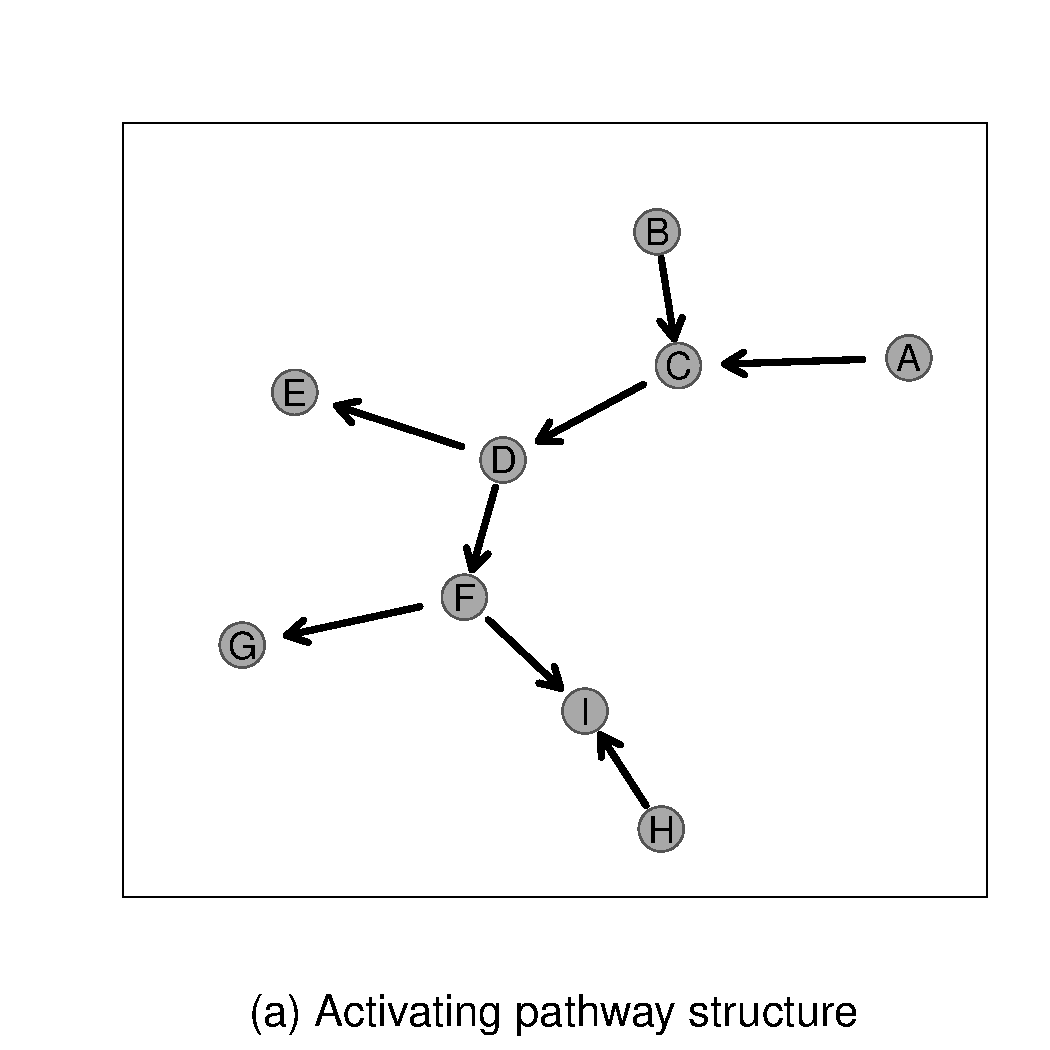
\includegraphics[width=.415\linewidth,height=.415\linewidth]{Plotsimple_graph-1} 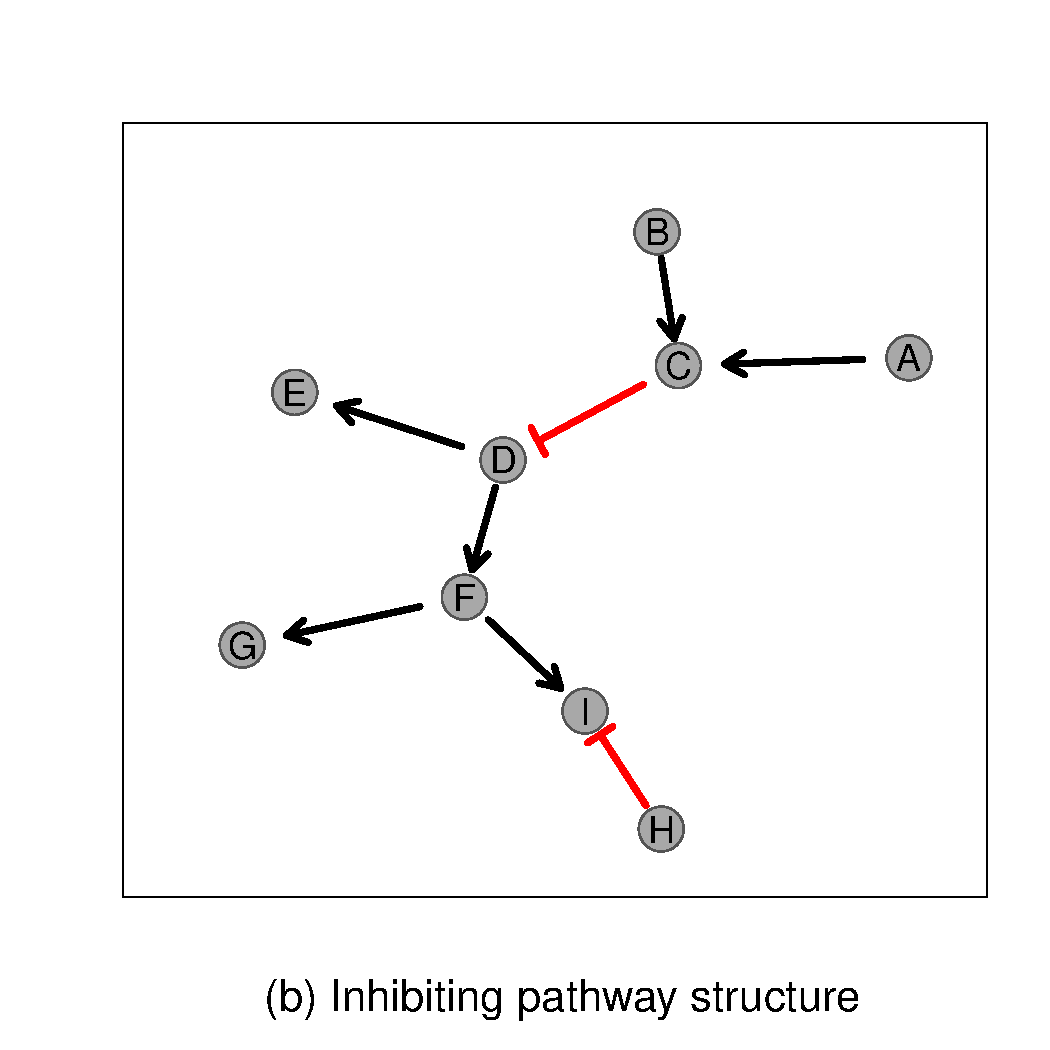
\includegraphics[width=.415\linewidth,height=.415\linewidth]{Plotsimple_graph-2} 

}

\caption{\textbf{Simulated graph structures}. A constructed graph structure used as an example to demonstrate the simulation procedure in Figures 2 and 3. Activating links are denoted by black arrows and inhibiting links by red edges. Inhibiting edges have been highlighted in red.}\label{fig:simple_graph}
\end{figure}

\hypertarget{sec:graphsim_demo}{%
\subsection{Generating a Simulated Expression
Dataset}\label{sec:graphsim_demo}}

The correlation parameter of \(\rho = 0.8\) is used to demonstrate the
inter-correlated datasets using a geometrically-generated relationship
matrix (as used for the example in
Figure~\protect\hyperlink{fig:simulation_activating:third}{2c}). This
\(\Sigma\) matrix was then used to sample from a multivariate normal
distribution such that each gene had a mean of \(0\), standard deviation
\(1\), and covariance within the range \([0,1]\) so that the
off-diagonal elements of \(\Sigma\) represent correlations. This
procedure generated a simulated (continuous normally-distributed)
log-expression profile for each node
(Figure~\protect\hyperlink{fig:simulation_activating:fourth}{2e}) with a
corresponding correlation structure
(Figure~\protect\hyperlink{fig:simulation_activating:fifth}{2d}). The
simulated correlation structure closely resembled the expected
correlation structure (\(\Sigma\) in
Figure~\protect\hyperlink{fig:simulation_activating:third}{2c}) even for
the relatively modest sample size (\(N=100\)) illustrated in
Figure~\protect\hyperlink{fig:simulation_activating}{2}. Once a gene
expression dataset comprising multiple pathways has been generated (as
in Figure~\protect\hyperlink{fig:simulation_activating:fourth}{2e}), it
can then be used to test procedures designed for analysis of empirical
gene expression data (such as those generated by microarrays or RNA-Seq)
that have been normalised on a log-scale.

The simulated dataset can be generated using the following code:

\begin{Shaded}
\begin{Highlighting}[]
\CommentTok{# activating graph}
\NormalTok{state <-}\StringTok{ }\KeywordTok{rep}\NormalTok{(}\DecValTok{1}\NormalTok{, }\KeywordTok{length}\NormalTok{(}\KeywordTok{E}\NormalTok{(graph)))}
\KeywordTok{plot_directed}\NormalTok{(graph, }\DataTypeTok{state=}\NormalTok{state, }\DataTypeTok{layout =}\NormalTok{ layout.kamada.kawai,}
              \DataTypeTok{cex.node=}\DecValTok{2}\NormalTok{, }\DataTypeTok{cex.arrow=}\DecValTok{4}\NormalTok{, }\DataTypeTok{arrow_clip =} \FloatTok{0.2}\NormalTok{)}
\KeywordTok{mtext}\NormalTok{(}\DataTypeTok{text =} \StringTok{"(a) Activating pathway structure"}\NormalTok{, }\DataTypeTok{side=}\DecValTok{1}\NormalTok{, }\DataTypeTok{line=}\FloatTok{3.5}\NormalTok{, }\DataTypeTok{at=}\FloatTok{0.075}\NormalTok{, }\DataTypeTok{adj=}\FloatTok{0.5}\NormalTok{, }\DataTypeTok{cex=}\FloatTok{1.75}\NormalTok{)}
\KeywordTok{box}\NormalTok{()}

\CommentTok{#adjacency matrix}
\NormalTok{adj_mat <-}\StringTok{ }\KeywordTok{make_adjmatrix_graph}\NormalTok{(graph)}

\CommentTok{#relationship matrix}
\NormalTok{dist_mat <-}\StringTok{ }\KeywordTok{make_distance_graph}\NormalTok{(graph, }\DataTypeTok{absolute =} \OtherTok{FALSE}\NormalTok{)}

\CommentTok{#sigma matrix directly from graph}
\NormalTok{sigma_mat <-}\StringTok{ }\KeywordTok{make_sigma_mat_dist_graph}\NormalTok{(graph, }\FloatTok{0.8}\NormalTok{, }\DataTypeTok{absolute =} \OtherTok{FALSE}\NormalTok{)}

\CommentTok{#show shortest paths of graph}
\NormalTok{shortest_paths <-}\StringTok{ }\KeywordTok{shortest.paths}\NormalTok{(graph)}

\CommentTok{#generate expression data directly from graph}
\NormalTok{expr <-}\StringTok{ }\KeywordTok{generate_expression}\NormalTok{(}\DecValTok{100}\NormalTok{, graph, }\DataTypeTok{cor =} \FloatTok{0.8}\NormalTok{, }\DataTypeTok{mean =} \DecValTok{0}\NormalTok{, }\DataTypeTok{comm =} \OtherTok{FALSE}\NormalTok{,}
                            \DataTypeTok{dist =} \OtherTok{TRUE}\NormalTok{, }\DataTypeTok{absolute =} \OtherTok{FALSE}\NormalTok{, }\DataTypeTok{state =}\NormalTok{ state)}
\CommentTok{#> Warning in generate_expression(100, graph, cor = 0.8, mean = 0,}
\CommentTok{#> comm = FALSE, : sigma matrix was not positive definite, nearest}
\CommentTok{#> approximation used.}

\CommentTok{#plot relationship matrix}
\KeywordTok{heatmap.2}\NormalTok{(}\KeywordTok{make_distance_graph}\NormalTok{(graph, }\DataTypeTok{absolute =} \OtherTok{FALSE}\NormalTok{),}
          \DataTypeTok{scale =} \StringTok{"none"}\NormalTok{, }\DataTypeTok{trace =} \StringTok{"none"}\NormalTok{, }\DataTypeTok{col =} \KeywordTok{colorpanel}\NormalTok{(}\DecValTok{50}\NormalTok{, }\StringTok{"white"}\NormalTok{, }\StringTok{"red"}\NormalTok{),}
\DataTypeTok{colsep =} \DecValTok{1}\OperatorTok{:}\KeywordTok{length}\NormalTok{(}\KeywordTok{V}\NormalTok{(graph)), }\DataTypeTok{rowsep =} \DecValTok{1}\OperatorTok{:}\KeywordTok{length}\NormalTok{(}\KeywordTok{V}\NormalTok{(graph)))}
\KeywordTok{mtext}\NormalTok{(}\DataTypeTok{text =} \StringTok{"(b) relationship matrix"}\NormalTok{, }\DataTypeTok{side=}\DecValTok{1}\NormalTok{, }\DataTypeTok{line=}\FloatTok{3.5}\NormalTok{, }\DataTypeTok{at=}\DecValTok{0}\NormalTok{, }\DataTypeTok{adj=}\FloatTok{0.5}\NormalTok{, }\DataTypeTok{cex=}\FloatTok{1.75}\NormalTok{)}

\CommentTok{#plot sigma matrix}
\KeywordTok{heatmap.2}\NormalTok{(}\KeywordTok{make_sigma_mat_dist_graph}\NormalTok{(graph, }\FloatTok{0.8}\NormalTok{, }\DataTypeTok{absolute =} \OtherTok{FALSE}\NormalTok{),}
\DataTypeTok{scale =} \StringTok{"none"}\NormalTok{, }\DataTypeTok{trace =} \StringTok{"none"}\NormalTok{, }\DataTypeTok{col =} \KeywordTok{colorpanel}\NormalTok{(}\DecValTok{50}\NormalTok{, }\StringTok{"white"}\NormalTok{, }\StringTok{"red"}\NormalTok{),}
\DataTypeTok{colsep =} \DecValTok{1}\OperatorTok{:}\KeywordTok{length}\NormalTok{(}\KeywordTok{V}\NormalTok{(graph)), }\DataTypeTok{rowsep =} \DecValTok{1}\OperatorTok{:}\KeywordTok{length}\NormalTok{(}\KeywordTok{V}\NormalTok{(graph)))}
\KeywordTok{mtext}\NormalTok{(}\DataTypeTok{text =} \KeywordTok{expression}\NormalTok{(}\KeywordTok{paste}\NormalTok{(}\StringTok{"(c) "}\NormalTok{, Sigma, }\StringTok{" matrix"}\NormalTok{)), }\DataTypeTok{side=}\DecValTok{1}\NormalTok{, }\DataTypeTok{line=}\FloatTok{3.5}\NormalTok{, }\DataTypeTok{at=}\DecValTok{0}\NormalTok{, }\DataTypeTok{adj=}\FloatTok{0.5}\NormalTok{, }\DataTypeTok{cex=}\FloatTok{1.75}\NormalTok{)}

\CommentTok{#simulated data}
\NormalTok{expr <-}\StringTok{ }\KeywordTok{generate_expression}\NormalTok{(}\DecValTok{100}\NormalTok{, graph, }\DataTypeTok{cor =} \FloatTok{0.8}\NormalTok{, }\DataTypeTok{mean =} \DecValTok{0}\NormalTok{,}
\DataTypeTok{comm =} \OtherTok{FALSE}\NormalTok{, }\DataTypeTok{dist =}\OtherTok{TRUE}\NormalTok{, }\DataTypeTok{absolute =} \OtherTok{FALSE}\NormalTok{, }\DataTypeTok{state =}\NormalTok{ state)}
\CommentTok{#> Warning in generate_expression(100, graph, cor = 0.8, mean = 0,}
\CommentTok{#> comm = FALSE, : sigma matrix was not positive definite, nearest}
\CommentTok{#> approximation used.}

\CommentTok{#plot simulated correlations}
\KeywordTok{heatmap.2}\NormalTok{(}\KeywordTok{cor}\NormalTok{(}\KeywordTok{t}\NormalTok{(expr)), }\DataTypeTok{scale =} \StringTok{"none"}\NormalTok{, }\DataTypeTok{trace =} \StringTok{"none"}\NormalTok{, }\DataTypeTok{col =} \KeywordTok{colorpanel}\NormalTok{(}\DecValTok{50}\NormalTok{, }\StringTok{"white"}\NormalTok{, }\StringTok{"red"}\NormalTok{),}
\DataTypeTok{colsep =} \DecValTok{1}\OperatorTok{:}\KeywordTok{length}\NormalTok{(}\KeywordTok{V}\NormalTok{(graph)), }\DataTypeTok{rowsep =} \DecValTok{1}\OperatorTok{:}\KeywordTok{length}\NormalTok{(}\KeywordTok{V}\NormalTok{(graph)))}
\KeywordTok{mtext}\NormalTok{(}\DataTypeTok{text =} \StringTok{"(d) Simulated correlation"}\NormalTok{, }\DataTypeTok{side=}\DecValTok{1}\NormalTok{, }\DataTypeTok{line=}\FloatTok{3.5}\NormalTok{, }\DataTypeTok{at=}\DecValTok{0}\NormalTok{, }\DataTypeTok{adj=}\FloatTok{0.5}\NormalTok{, }\DataTypeTok{cex=}\FloatTok{1.75}\NormalTok{)}

\CommentTok{#plot simulated expression data}
\KeywordTok{heatmap.2}\NormalTok{(expr, }\DataTypeTok{scale =} \StringTok{"none"}\NormalTok{, }\DataTypeTok{trace =} \StringTok{"none"}\NormalTok{, }\DataTypeTok{col =} \KeywordTok{bluered}\NormalTok{(}\DecValTok{50}\NormalTok{),}
\DataTypeTok{colsep =} \DecValTok{1}\OperatorTok{:}\KeywordTok{length}\NormalTok{(}\KeywordTok{V}\NormalTok{(graph)), }\DataTypeTok{rowsep =} \DecValTok{1}\OperatorTok{:}\KeywordTok{length}\NormalTok{(}\KeywordTok{V}\NormalTok{(graph)), }\DataTypeTok{labCol =} \StringTok{""}\NormalTok{)}
\KeywordTok{mtext}\NormalTok{(}\DataTypeTok{text =} \StringTok{"samples"}\NormalTok{, }\DataTypeTok{side=}\DecValTok{1}\NormalTok{, }\DataTypeTok{line=}\FloatTok{1.5}\NormalTok{, }\DataTypeTok{at=}\FloatTok{0.2}\NormalTok{, }\DataTypeTok{adj=}\FloatTok{0.5}\NormalTok{, }\DataTypeTok{cex=}\FloatTok{1.5}\NormalTok{)}
\KeywordTok{mtext}\NormalTok{(}\DataTypeTok{text =} \StringTok{"genes"}\NormalTok{, }\DataTypeTok{side=}\DecValTok{4}\NormalTok{, }\DataTypeTok{line=}\DecValTok{1}\NormalTok{, }\DataTypeTok{at=}\OperatorTok{-}\FloatTok{0.4}\NormalTok{, }\DataTypeTok{adj=}\FloatTok{0.5}\NormalTok{, }\DataTypeTok{cex=}\FloatTok{1.5}\NormalTok{)}
\KeywordTok{mtext}\NormalTok{(}\DataTypeTok{text =} \StringTok{"(e) Simulated expression data (log scale)"}\NormalTok{, }\DataTypeTok{side=}\DecValTok{1}\NormalTok{, }\DataTypeTok{line=}\FloatTok{3.5}\NormalTok{, }\DataTypeTok{at=}\DecValTok{0}\NormalTok{, }\DataTypeTok{adj=}\FloatTok{0.5}\NormalTok{, }\DataTypeTok{cex=}\FloatTok{1.75}\NormalTok{)}
\end{Highlighting}
\end{Shaded}

\begin{figure}

{\centering 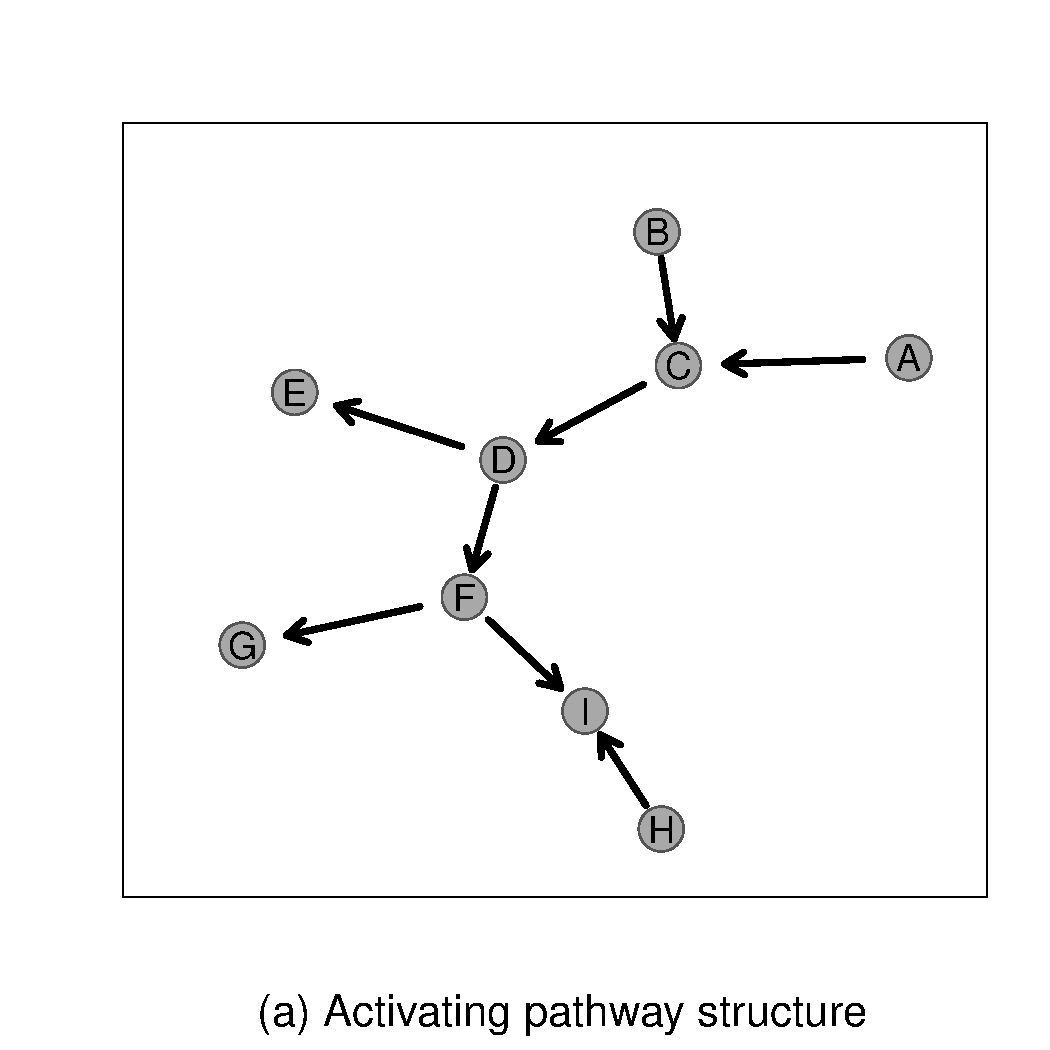
\includegraphics[width=.415\linewidth,height=.415\linewidth]{Plotsimulation_activating-1} 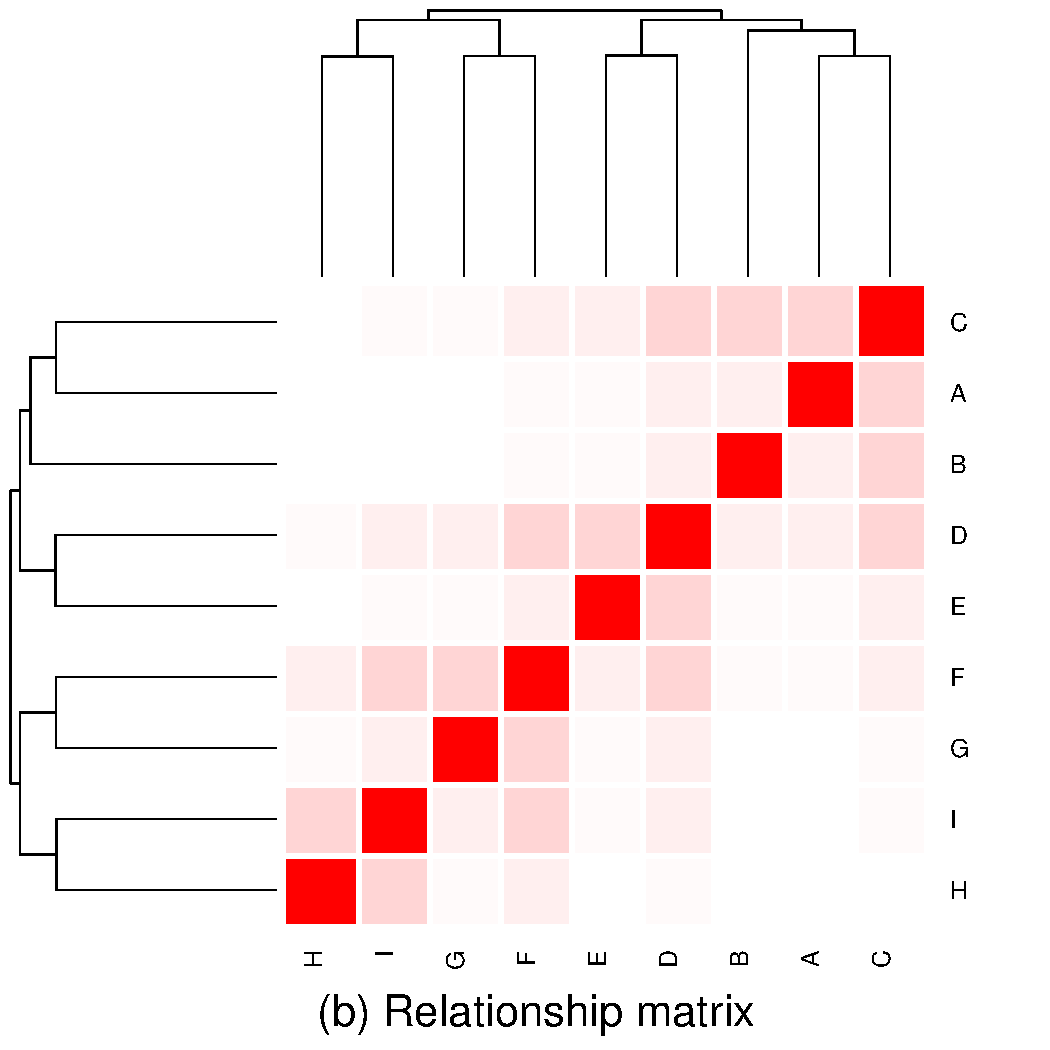
\includegraphics[width=.415\linewidth,height=.415\linewidth]{Plotsimulation_activating-2} 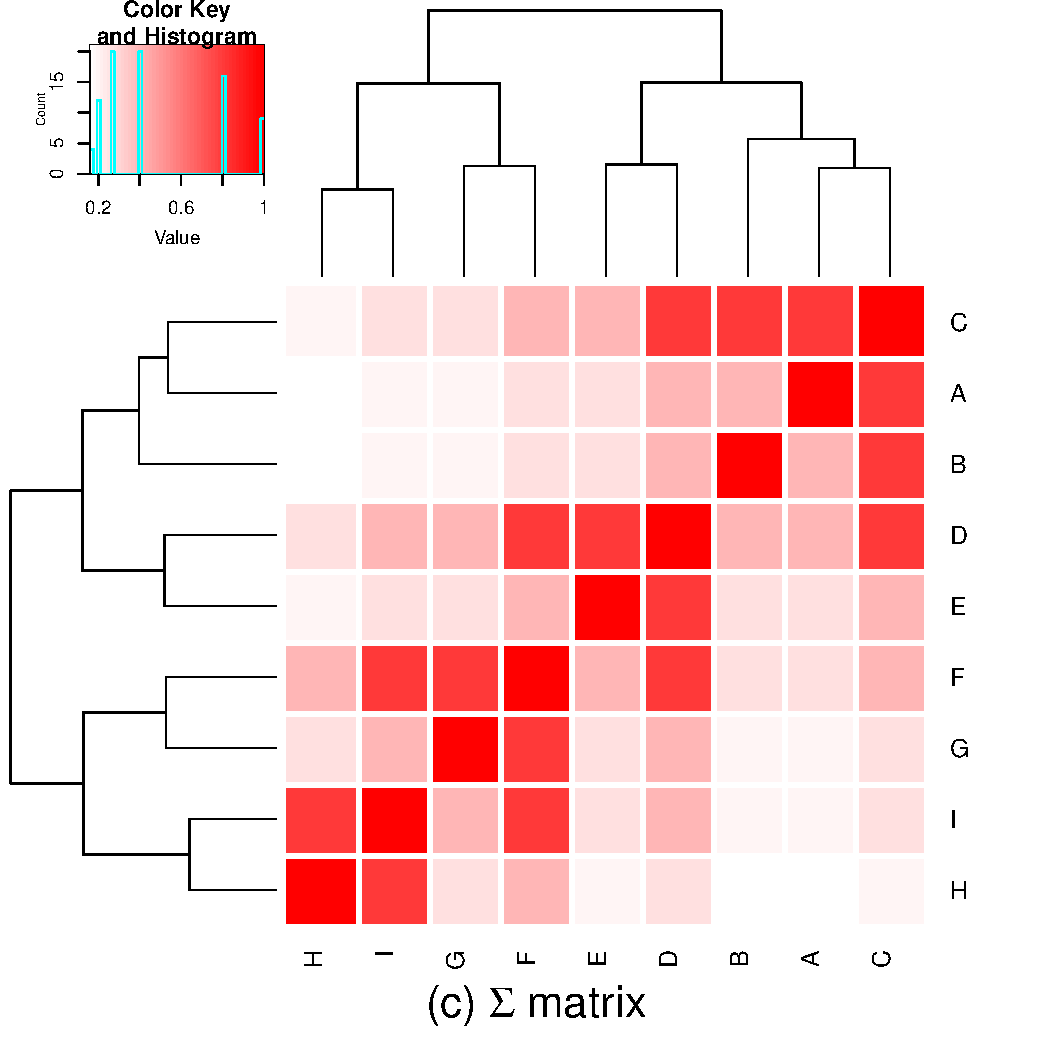
\includegraphics[width=.415\linewidth,height=.415\linewidth]{Plotsimulation_activating-3} 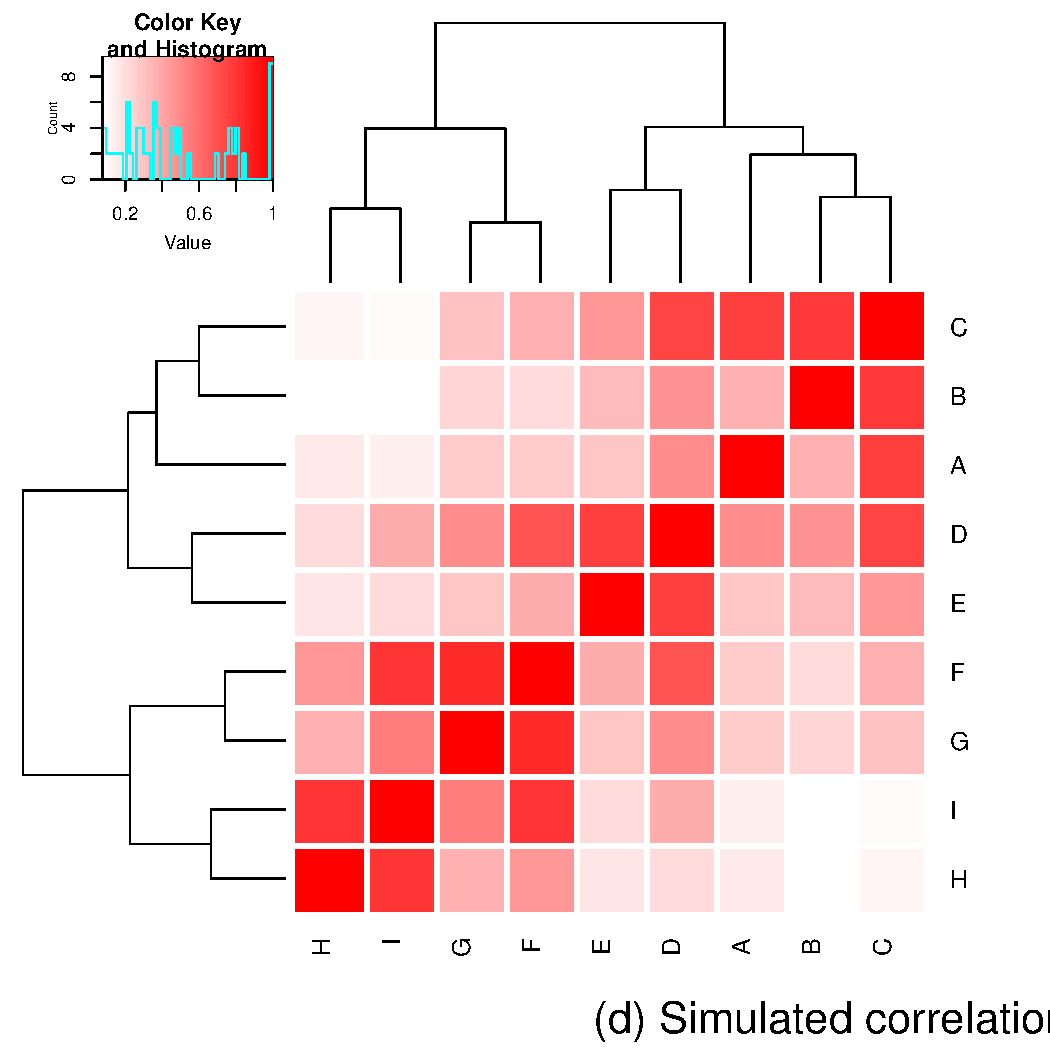
\includegraphics[width=.415\linewidth,height=.415\linewidth]{Plotsimulation_activating-4} 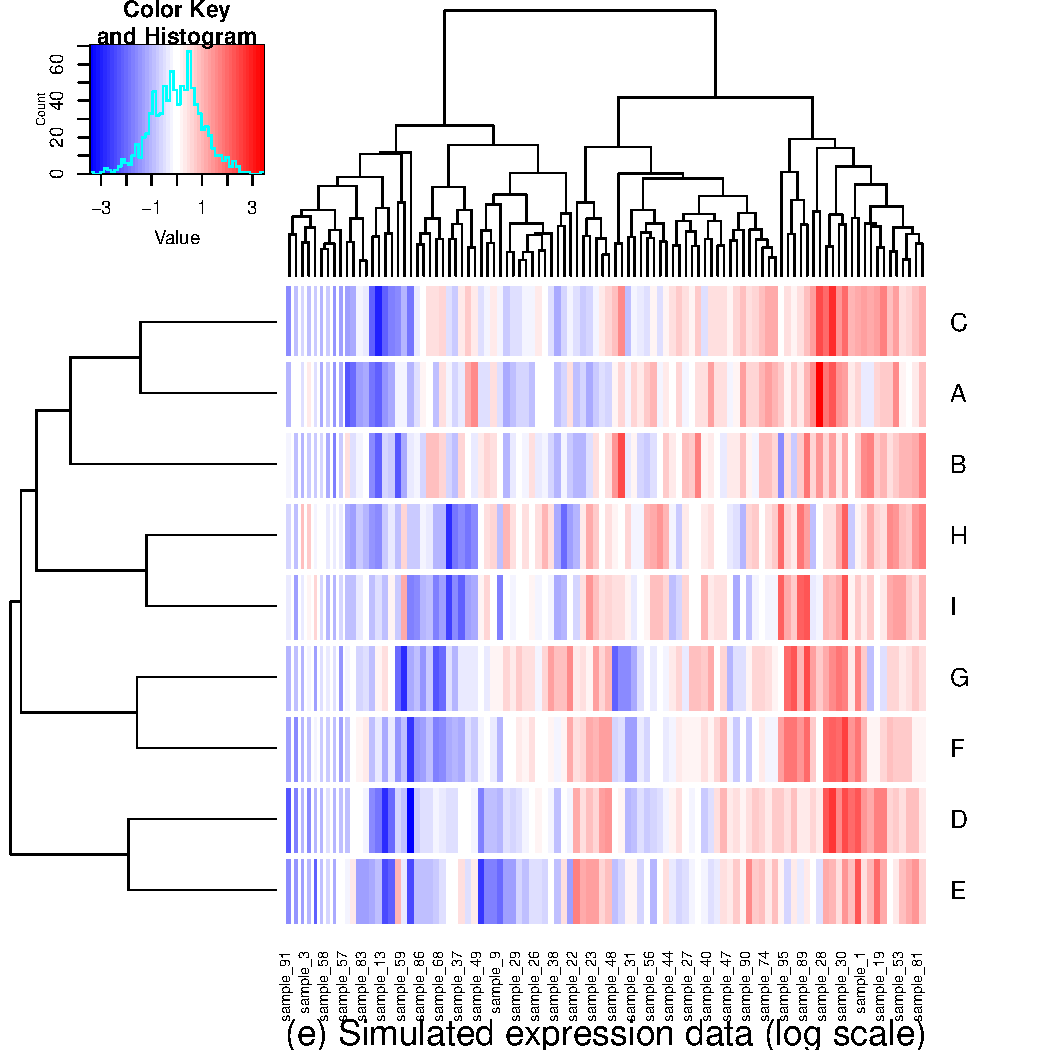
\includegraphics[width=.830\linewidth,height=.415\linewidth]{Plotsimulation_activating-5} 

}

\caption{\textbf{Simulating expression from a graph structure}. An example of a graph structure (a) that has been used to derive a relationship matrix (b), $\Sigma$  matrix (c) and correlation structure (d) from the relative distances between the nodes. Non-negative values are coloured white to red from $0$ to $1$. This $\Sigma$ matrix has been used to generate a simulated expression dataset of 100 samples (coloured blue to red from low to high) via sampling from the multivariate normal distribution. Here genes with closer relationships in the pathway structure show a higher correlation between simulated values.}\label{fig:simulation_activating}
\end{figure}

The simulation procedure
(Figure~\protect\hyperlink{fig:simulation_activating}{2}) can similarly
be used for pathways containing inhibitory links
(Figure~\protect\hyperlink{fig:simulation_inhibiting}{3}) with several
refinements. With the inhibitory links
(Figure~\protect\hyperlink{fig:simulation_inhibiting:first}{3a}),
distances are calculated in the same manner as before
(Figure~\protect\hyperlink{fig:simulation_inhibiting:second}{3b}) with
inhibitions accounted for by iteratively multiplying downstream nodes by
\(-1\) to form modules with negative correlations between them
(Figures~\protect\hyperlink{fig:simulation_inhibiting:third}{3c}
and~\protect\hyperlink{fig:simulation_inhibiting:fifth}{3d}). A
multivariate normal distribution with these negative correlations can be
sampled to generate simulated data
(Figure~\protect\hyperlink{fig:simulation_inhibiting:fourth}{3e}).

\begin{Shaded}
\begin{Highlighting}[]

\CommentTok{#generate parameters for inhibitions}
\NormalTok{state <-}\StringTok{ }\KeywordTok{c}\NormalTok{(}\DecValTok{1}\NormalTok{, }\DecValTok{1}\NormalTok{, }\DecValTok{-1}\NormalTok{, }\DecValTok{1}\NormalTok{, }\DecValTok{1}\NormalTok{, }\DecValTok{1}\NormalTok{, }\DecValTok{1}\NormalTok{, }\DecValTok{-1}\NormalTok{)}
\KeywordTok{plot_directed}\NormalTok{(graph, }\DataTypeTok{state=}\NormalTok{state, }\DataTypeTok{layout =}\NormalTok{ layout.kamada.kawai,}
              \DataTypeTok{cex.node=}\DecValTok{2}\NormalTok{, }\DataTypeTok{cex.arrow=}\DecValTok{4}\NormalTok{, }\DataTypeTok{arrow_clip =} \FloatTok{0.2}\NormalTok{)}
\KeywordTok{mtext}\NormalTok{(}\DataTypeTok{text =} \StringTok{"(a) Inhibiting pathway structure"}\NormalTok{, }\DataTypeTok{side=}\DecValTok{1}\NormalTok{, }\DataTypeTok{line=}\FloatTok{3.5}\NormalTok{, }\DataTypeTok{at=}\FloatTok{0.075}\NormalTok{, }\DataTypeTok{adj=}\FloatTok{0.5}\NormalTok{, }\DataTypeTok{cex=}\FloatTok{1.75}\NormalTok{)}
\KeywordTok{box}\NormalTok{()}

\CommentTok{#adjacency matrix}
\NormalTok{adj_mat <-}\StringTok{ }\KeywordTok{make_adjmatrix_graph}\NormalTok{(graph)}

\CommentTok{#relationship matrix}
\NormalTok{dist_mat <-}\StringTok{ }\KeywordTok{make_distance_graph}\NormalTok{(graph, }\DataTypeTok{absolute =} \OtherTok{FALSE}\NormalTok{)}

\CommentTok{#sigma matrix directly from graph}
\NormalTok{sigma_mat <-}\StringTok{ }\KeywordTok{make_sigma_mat_dist_graph}\NormalTok{(graph, }\DataTypeTok{state =}\NormalTok{ state, }\FloatTok{0.8}\NormalTok{, }\DataTypeTok{absolute =} \OtherTok{FALSE}\NormalTok{)}

\CommentTok{#show shortest paths of graph}
\NormalTok{shortest_paths <-}\StringTok{ }\KeywordTok{shortest.paths}\NormalTok{(graph)}

\CommentTok{#generate expression data directly from graph}
\NormalTok{expr <-}\StringTok{ }\KeywordTok{generate_expression}\NormalTok{(}\DecValTok{100}\NormalTok{, graph, }\DataTypeTok{state =}\NormalTok{ state, }\DataTypeTok{cor =} \FloatTok{0.8}\NormalTok{, }\DataTypeTok{mean =} \DecValTok{0}\NormalTok{, }\DataTypeTok{comm =} \OtherTok{FALSE}\NormalTok{,}
                            \DataTypeTok{dist =} \OtherTok{TRUE}\NormalTok{, }\DataTypeTok{absolute =} \OtherTok{FALSE}\NormalTok{)}
\CommentTok{#> Warning in generate_expression(100, graph, state = state, cor =}
\CommentTok{#> 0.8, mean = 0, : sigma matrix was not positive definite, nearest}
\CommentTok{#> approximation used.}

\CommentTok{#plot relationship matrix}
\KeywordTok{heatmap.2}\NormalTok{(}\KeywordTok{make_distance_graph}\NormalTok{(graph, }\DataTypeTok{absolute =} \OtherTok{FALSE}\NormalTok{),}
          \DataTypeTok{scale =} \StringTok{"none"}\NormalTok{, }\DataTypeTok{trace =} \StringTok{"none"}\NormalTok{, }\DataTypeTok{col =} \KeywordTok{colorpanel}\NormalTok{(}\DecValTok{50}\NormalTok{, }\StringTok{"white"}\NormalTok{, }\StringTok{"red"}\NormalTok{),}
\DataTypeTok{colsep =} \DecValTok{1}\OperatorTok{:}\KeywordTok{length}\NormalTok{(}\KeywordTok{V}\NormalTok{(graph)), }\DataTypeTok{rowsep =} \DecValTok{1}\OperatorTok{:}\KeywordTok{length}\NormalTok{(}\KeywordTok{V}\NormalTok{(graph)))}
\KeywordTok{mtext}\NormalTok{(}\DataTypeTok{text =} \StringTok{"(b) relationship matrix"}\NormalTok{, }\DataTypeTok{side=}\DecValTok{1}\NormalTok{, }\DataTypeTok{line=}\FloatTok{3.5}\NormalTok{, }\DataTypeTok{at=}\DecValTok{0}\NormalTok{, }\DataTypeTok{adj=}\FloatTok{0.5}\NormalTok{, }\DataTypeTok{cex=}\FloatTok{1.75}\NormalTok{)}

\CommentTok{# #plot sigma matrix}
\KeywordTok{heatmap.2}\NormalTok{(}\KeywordTok{make_sigma_mat_dist_graph}\NormalTok{(graph, }\DataTypeTok{state =}\NormalTok{ state, }\FloatTok{0.8}\NormalTok{, }\DataTypeTok{absolute =} \OtherTok{FALSE}\NormalTok{),}
\DataTypeTok{scale =} \StringTok{"none"}\NormalTok{, }\DataTypeTok{trace =} \StringTok{"none"}\NormalTok{, }\DataTypeTok{col =} \KeywordTok{colorpanel}\NormalTok{(}\DecValTok{50}\NormalTok{, }\StringTok{"blue"}\NormalTok{, }\StringTok{"white"}\NormalTok{, }\StringTok{"red"}\NormalTok{),}
\DataTypeTok{colsep =} \DecValTok{1}\OperatorTok{:}\KeywordTok{length}\NormalTok{(}\KeywordTok{V}\NormalTok{(graph)), }\DataTypeTok{rowsep =} \DecValTok{1}\OperatorTok{:}\KeywordTok{length}\NormalTok{(}\KeywordTok{V}\NormalTok{(graph)))}
\KeywordTok{mtext}\NormalTok{(}\DataTypeTok{text =} \KeywordTok{expression}\NormalTok{(}\KeywordTok{paste}\NormalTok{(}\StringTok{"(c) "}\NormalTok{, Sigma, }\StringTok{" matrix"}\NormalTok{)), }\DataTypeTok{side=}\DecValTok{1}\NormalTok{, }\DataTypeTok{line=}\FloatTok{3.5}\NormalTok{, }\DataTypeTok{at=}\DecValTok{0}\NormalTok{, }\DataTypeTok{adj=}\FloatTok{0.5}\NormalTok{, }\DataTypeTok{cex=}\FloatTok{1.75}\NormalTok{)}

\CommentTok{#simulated data}
\NormalTok{expr <-}\StringTok{ }\KeywordTok{generate_expression}\NormalTok{(}\DecValTok{100}\NormalTok{, graph,  }\DataTypeTok{state =}\NormalTok{ state, }\DataTypeTok{cor =} \FloatTok{0.8}\NormalTok{, }\DataTypeTok{mean =} \DecValTok{0}\NormalTok{,}
\DataTypeTok{comm =} \OtherTok{FALSE}\NormalTok{, }\DataTypeTok{dist =}\OtherTok{TRUE}\NormalTok{, }\DataTypeTok{absolute =} \OtherTok{FALSE}\NormalTok{)}
\CommentTok{#> Warning in generate_expression(100, graph, state = state, cor =}
\CommentTok{#> 0.8, mean = 0, : sigma matrix was not positive definite, nearest}
\CommentTok{#> approximation used.}

\CommentTok{#plot simulated correlations}
\KeywordTok{heatmap.2}\NormalTok{(}\KeywordTok{cor}\NormalTok{(}\KeywordTok{t}\NormalTok{(expr)), }\DataTypeTok{scale =} \StringTok{"none"}\NormalTok{, }\DataTypeTok{trace =} \StringTok{"none"}\NormalTok{, }\DataTypeTok{col =} \KeywordTok{colorpanel}\NormalTok{(}\DecValTok{50}\NormalTok{, }\StringTok{"blue"}\NormalTok{, }\StringTok{"white"}\NormalTok{, }\StringTok{"red"}\NormalTok{),}
\DataTypeTok{colsep =} \DecValTok{1}\OperatorTok{:}\KeywordTok{length}\NormalTok{(}\KeywordTok{V}\NormalTok{(graph)), }\DataTypeTok{rowsep =} \DecValTok{1}\OperatorTok{:}\KeywordTok{length}\NormalTok{(}\KeywordTok{V}\NormalTok{(graph)))}
\KeywordTok{mtext}\NormalTok{(}\DataTypeTok{text =} \StringTok{"(d) Simulated correlation"}\NormalTok{, }\DataTypeTok{side=}\DecValTok{1}\NormalTok{, }\DataTypeTok{line=}\FloatTok{3.5}\NormalTok{, }\DataTypeTok{at=}\DecValTok{0}\NormalTok{, }\DataTypeTok{adj=}\FloatTok{0.5}\NormalTok{, }\DataTypeTok{cex=}\FloatTok{1.75}\NormalTok{)}

\CommentTok{#plot simulated expression data}
\KeywordTok{heatmap.2}\NormalTok{(expr, }\DataTypeTok{scale =} \StringTok{"none"}\NormalTok{, }\DataTypeTok{trace =} \StringTok{"none"}\NormalTok{, }\DataTypeTok{col =} \KeywordTok{bluered}\NormalTok{(}\DecValTok{50}\NormalTok{),}
\DataTypeTok{colsep =} \DecValTok{1}\OperatorTok{:}\KeywordTok{length}\NormalTok{(}\KeywordTok{V}\NormalTok{(graph)), }\DataTypeTok{rowsep =} \DecValTok{1}\OperatorTok{:}\KeywordTok{length}\NormalTok{(}\KeywordTok{V}\NormalTok{(graph)), }\DataTypeTok{labCol =} \StringTok{""}\NormalTok{)}
\KeywordTok{mtext}\NormalTok{(}\DataTypeTok{text =} \StringTok{"samples"}\NormalTok{, }\DataTypeTok{side=}\DecValTok{1}\NormalTok{, }\DataTypeTok{line=}\FloatTok{1.5}\NormalTok{, }\DataTypeTok{at=}\FloatTok{0.2}\NormalTok{, }\DataTypeTok{adj=}\FloatTok{0.5}\NormalTok{, }\DataTypeTok{cex=}\FloatTok{1.5}\NormalTok{)}
\KeywordTok{mtext}\NormalTok{(}\DataTypeTok{text =} \StringTok{"genes"}\NormalTok{, }\DataTypeTok{side=}\DecValTok{4}\NormalTok{, }\DataTypeTok{line=}\DecValTok{1}\NormalTok{, }\DataTypeTok{at=}\OperatorTok{-}\FloatTok{0.4}\NormalTok{, }\DataTypeTok{adj=}\FloatTok{0.5}\NormalTok{, }\DataTypeTok{cex=}\FloatTok{1.5}\NormalTok{)}
\KeywordTok{mtext}\NormalTok{(}\DataTypeTok{text =} \StringTok{"(e) Simulated expression data (log scale)"}\NormalTok{, }\DataTypeTok{side=}\DecValTok{1}\NormalTok{, }\DataTypeTok{line=}\FloatTok{3.5}\NormalTok{, }\DataTypeTok{at=}\DecValTok{0}\NormalTok{, }\DataTypeTok{adj=}\FloatTok{0.5}\NormalTok{, }\DataTypeTok{cex=}\FloatTok{1.75}\NormalTok{)}
\end{Highlighting}
\end{Shaded}

\begin{figure}

{\centering 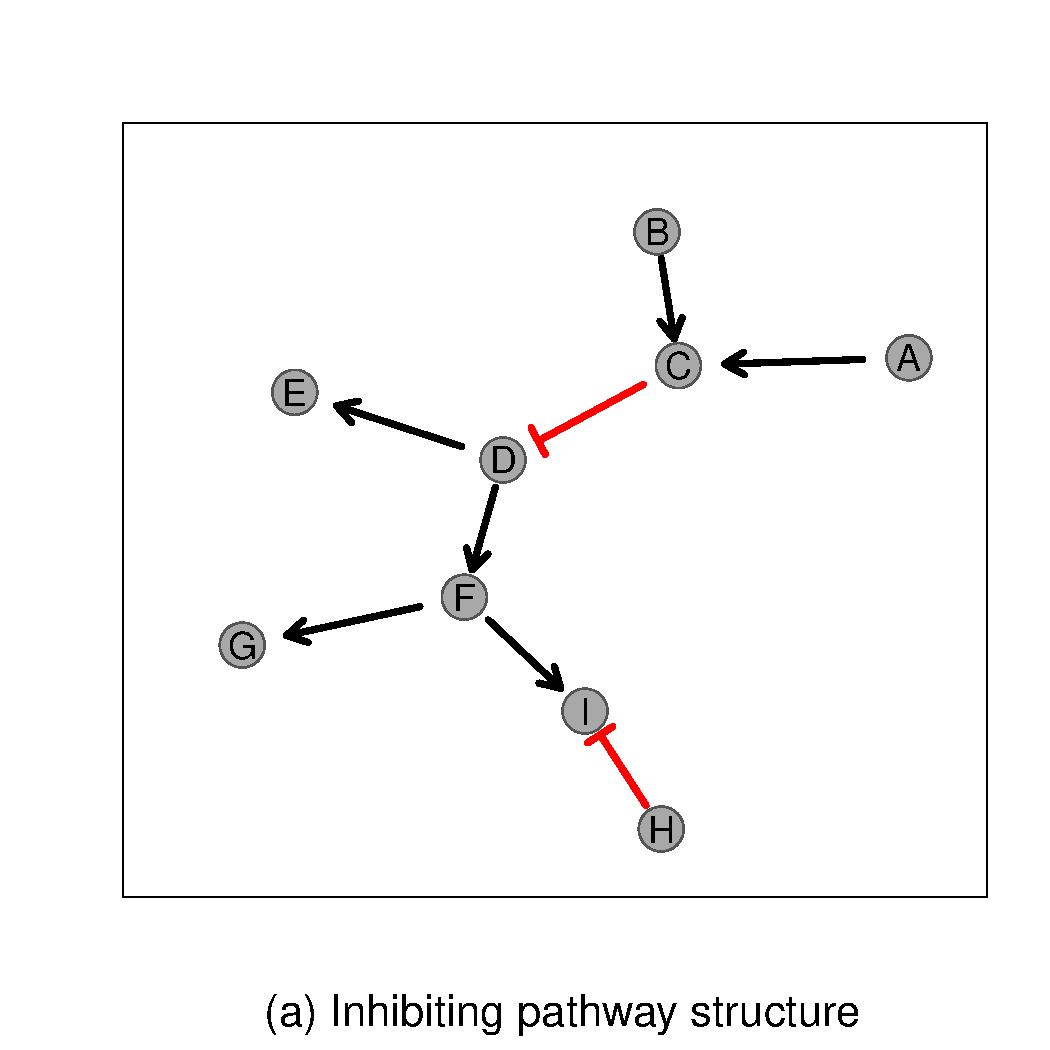
\includegraphics[width=.415\linewidth,height=.415\linewidth]{Plotsimulation_inhibiting-1} 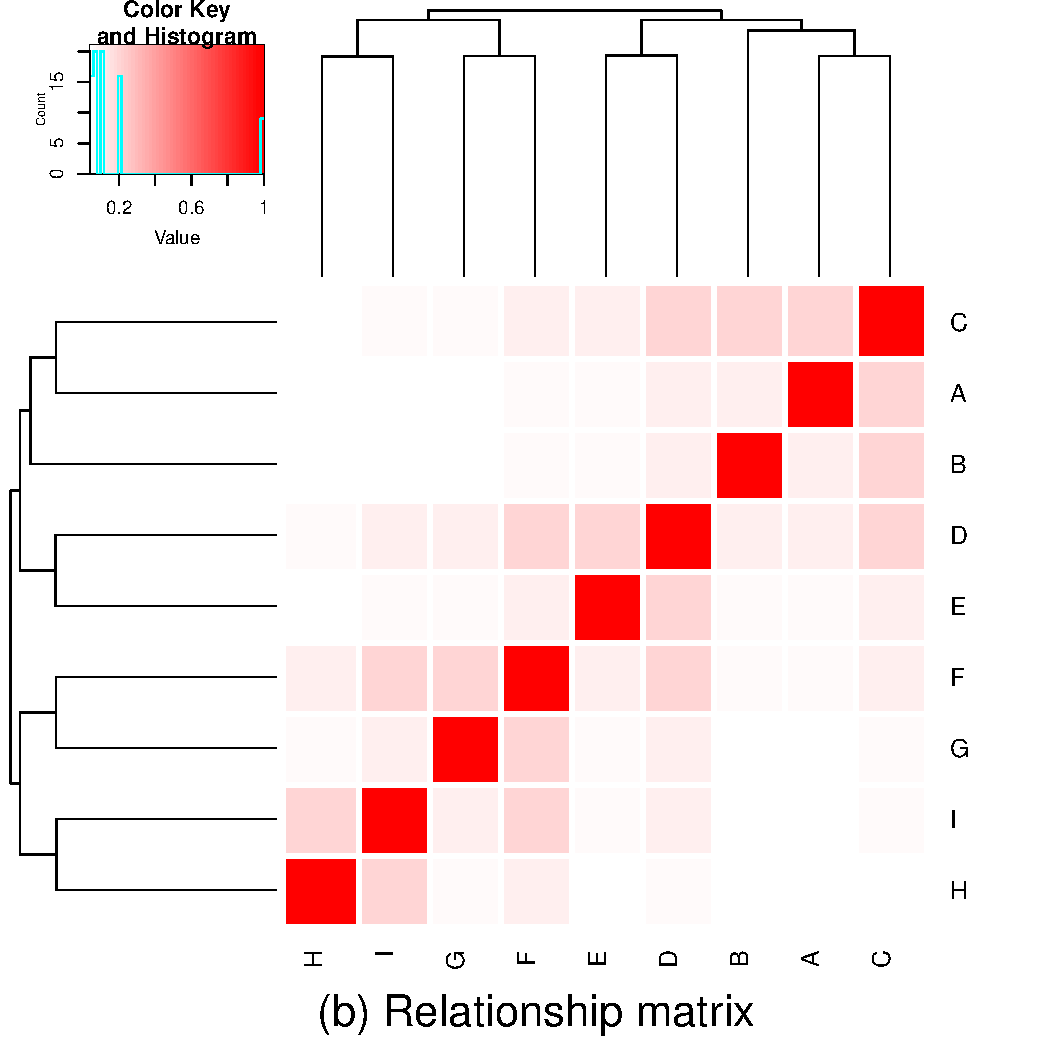
\includegraphics[width=.415\linewidth,height=.415\linewidth]{Plotsimulation_inhibiting-2} 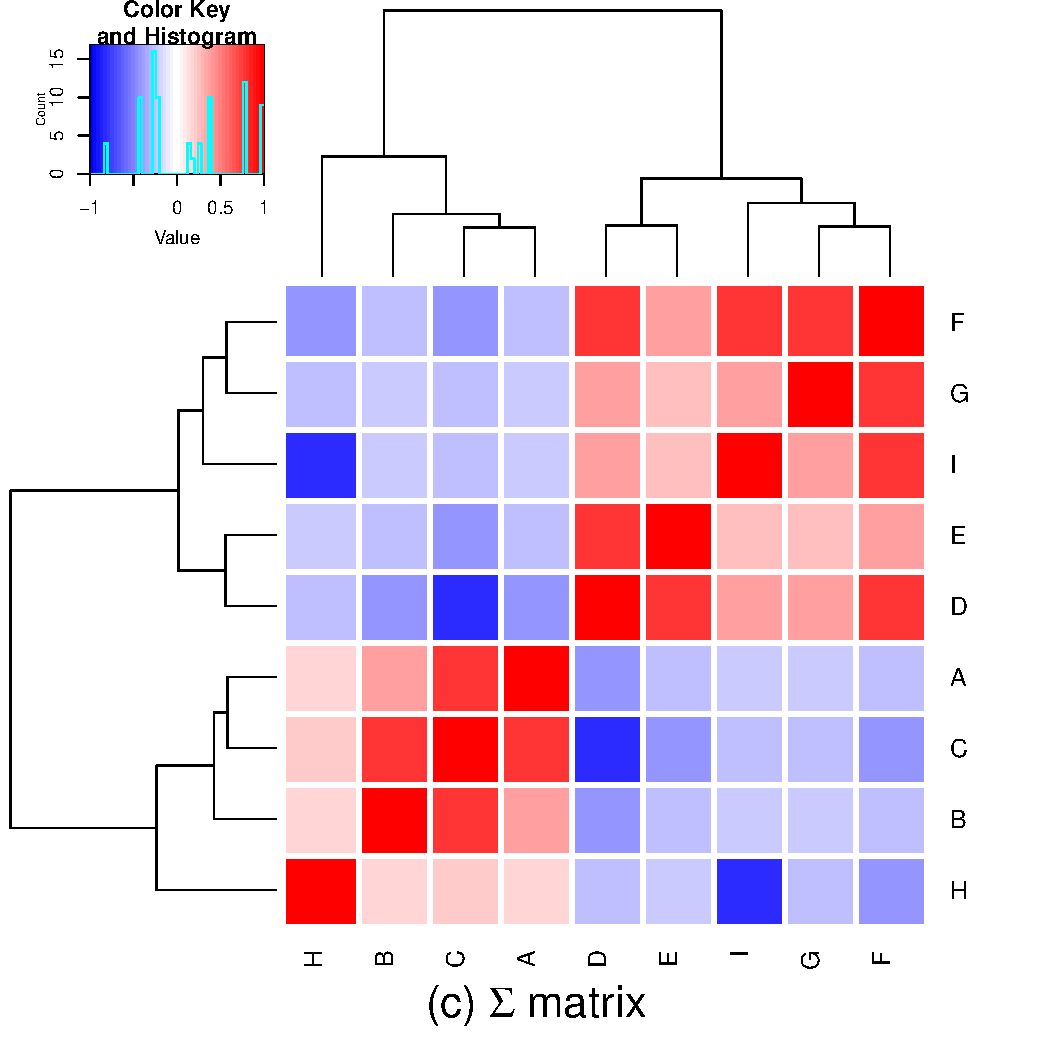
\includegraphics[width=.415\linewidth,height=.415\linewidth]{Plotsimulation_inhibiting-3} 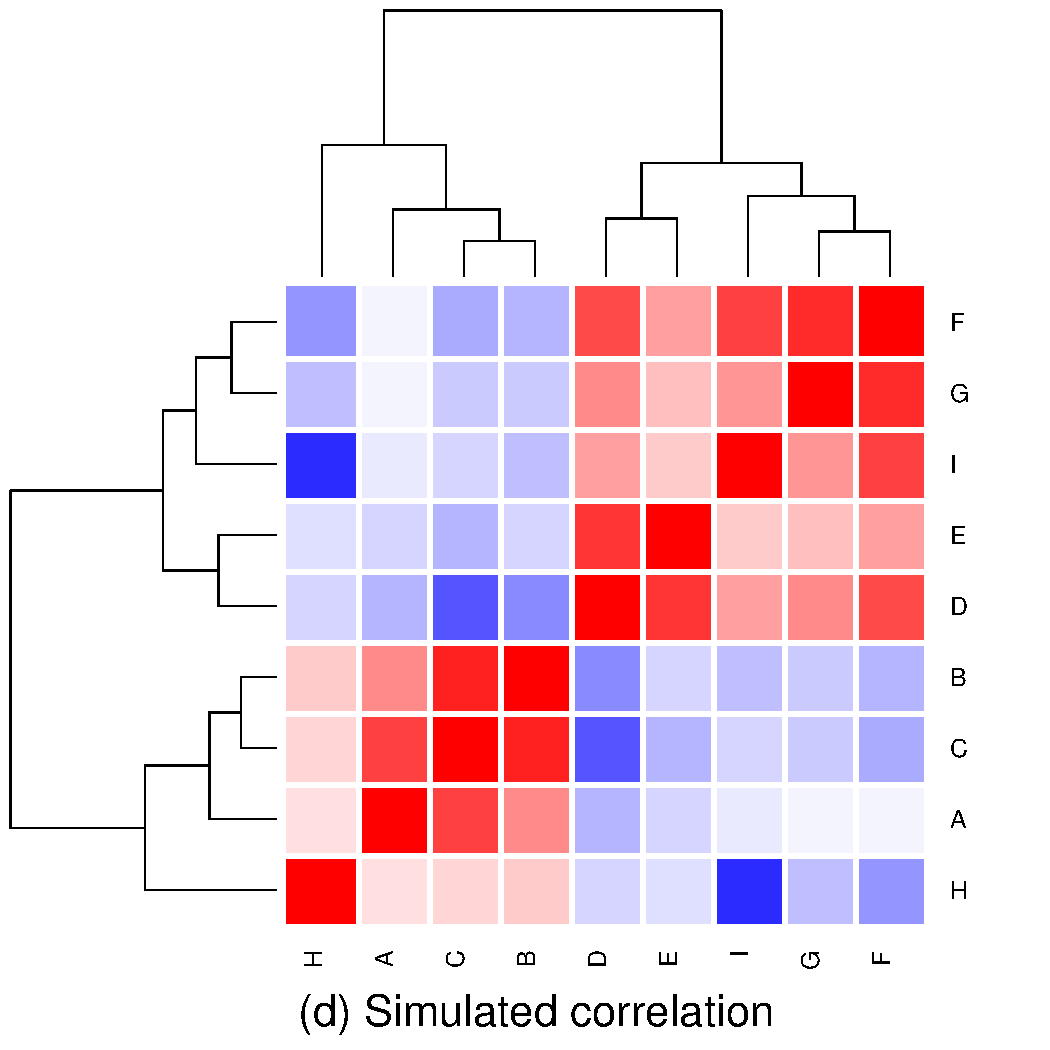
\includegraphics[width=.415\linewidth,height=.415\linewidth]{Plotsimulation_inhibiting-4} 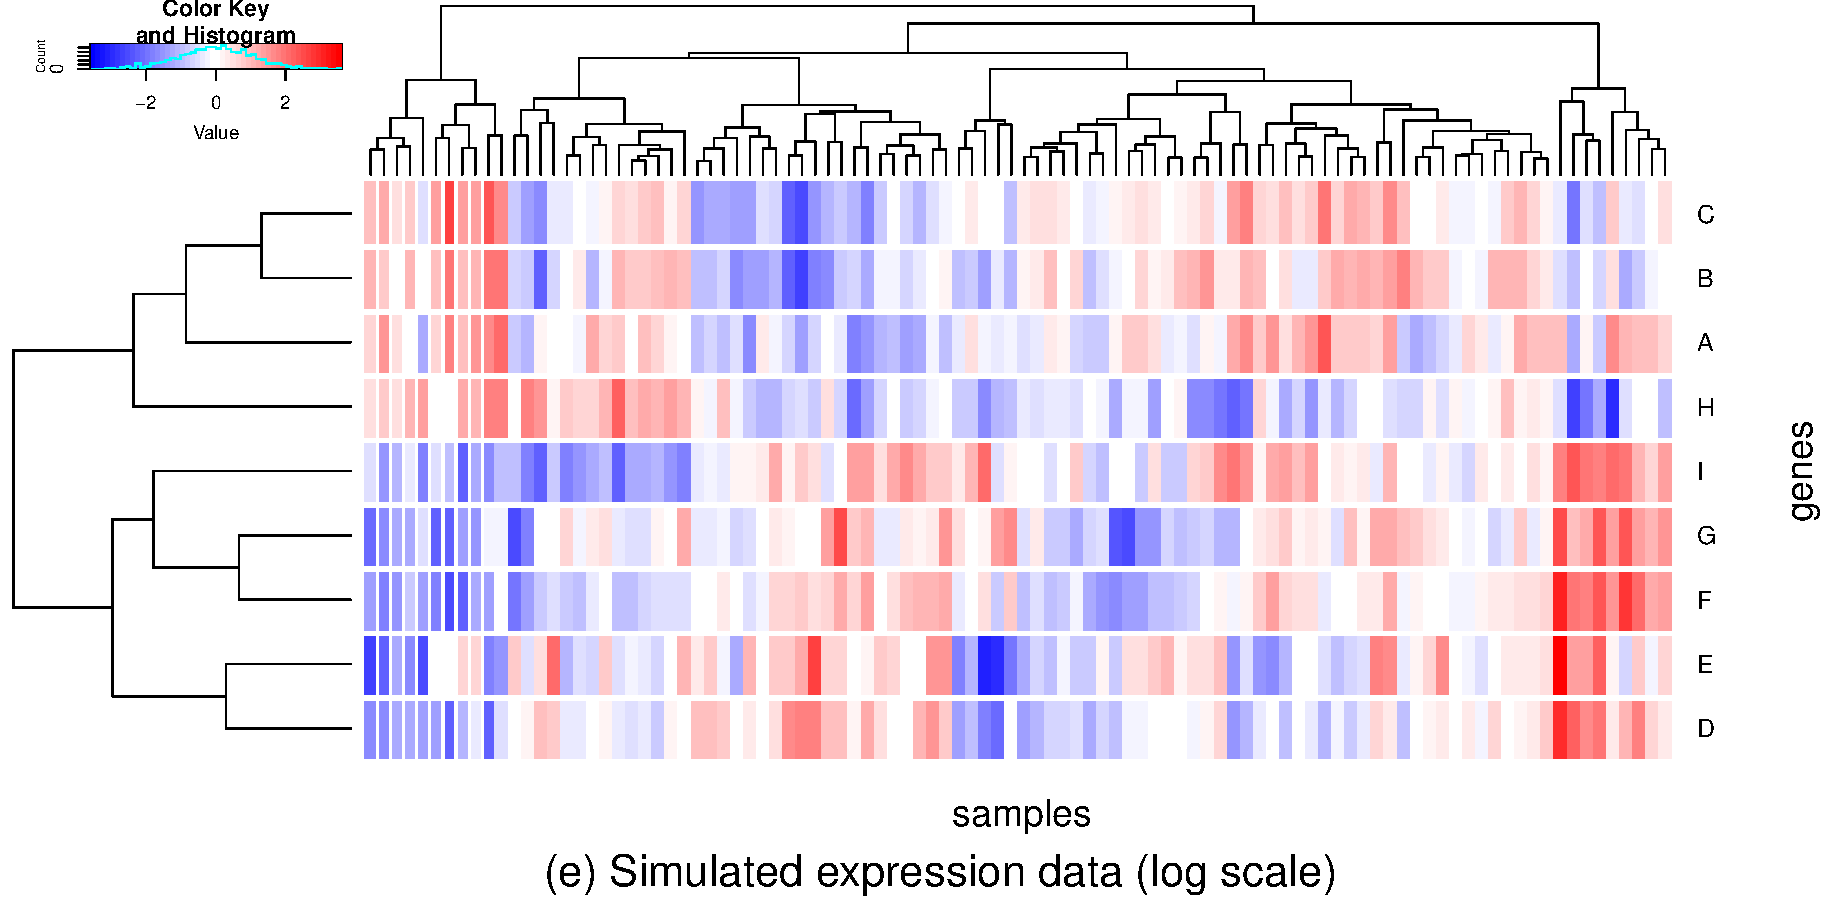
\includegraphics[width=.830\linewidth,height=.415\linewidth]{Plotsimulation_inhibiting-5} 

}

\caption{\textbf{Simulating expression from graph structure with inhibitions}. An example of a graph structure (a), that has been used to derive a relationship matrix (b), $\Sigma$ matrix (c), and correlation structure (d), from the relative distances between the nodes. These values are coloured blue to red from $-1$ to $1$. This has been used to generate a simulated expression dataset of 100 samples (coloured blue to red from low to high) via sampling from the multivariate normal distribution. Here the inhibitory relationships between genes are reflected in negatively correlated simulated  values.}\label{fig:simulation_inhibiting}
\end{figure}

The simulation procedure is also demonstrated here
(Figure~\protect\hyperlink{fig:simulation_smad}{4}) on a pathway
structure for a known biological pathway (from reactome R-HSA-2173789)
of TGF-\(\beta\) receptor signaling activates SMADs
(Figure~\protect\hyperlink{fig:simulation_smad:first}{4a}) derived from
the Reactome database version 52 \texttt{{[}@Reactome{]}}. Distances are
calculated in the same manner as before
(Figure~\protect\hyperlink{fig:simulation_smad:second}{4b}) producing
blocks of correlated genes
(Figures~\protect\hyperlink{fig:simulation_smad:third}{4c}
and~\protect\hyperlink{fig:simulation_smad:fifth}{4d}). This shows that
multivariate normal distribution can be sampled to generate simulated
data to represent expression with the complexity of a biological pathway
(Figure~\protect\hyperlink{fig:simulation_smad:fourth}{4e}). Here
\emph{SMAD7} exhibits negative correlations with the other SMADs
consistent with it's functions as as an ``inhibitor SMAD'' with
competitively inhibits \emph{SMAD4}.

\begin{Shaded}
\begin{Highlighting}[]

\CommentTok{#import graph from data}
\NormalTok{graph <-}\StringTok{ }\KeywordTok{identity}\NormalTok{(TGFBeta_Smad_graph)}

\CommentTok{#generate parameters for inhibitions}
\NormalTok{state <-}\StringTok{ }\KeywordTok{rep}\NormalTok{(}\DecValTok{1}\NormalTok{, }\KeywordTok{length}\NormalTok{(}\KeywordTok{E}\NormalTok{(graph)))}
\NormalTok{pathway <-}\StringTok{ }\KeywordTok{get.edgelist}\NormalTok{(graph)}
\NormalTok{state[pathway[,}\DecValTok{1}\NormalTok{] }\OperatorTok\StringTok{ }\KeywordTok{c}\NormalTok{(}\StringTok{"SMAD6"}\NormalTok{, }\StringTok{"SMAD7"}\NormalTok{, }\StringTok{"BAMBI"}\NormalTok{, }\StringTok{"SMURF1"}\NormalTok{, }\StringTok{"SMURF2"}\NormalTok{, }\StringTok{"UCHL5"}\NormalTok{, }\StringTok{"USP15"}\NormalTok{, }\StringTok{"UBB"}\NormalTok{, }\StringTok{"UBC"}\NormalTok{, }\StringTok{"PMEPA1"}\NormalTok{, }\StringTok{"PPP1CA"}\NormalTok{, }\StringTok{"PPP1CB"}\NormalTok{, }\StringTok{"PPP1CC"}\NormalTok{, }\StringTok{"PPP1R15A"}\NormalTok{)] <-}\StringTok{ }\DecValTok{2}
\NormalTok{state[}\KeywordTok{is.na}\NormalTok{(state)] <-}\StringTok{ }\DecValTok{1}

\KeywordTok{plot_directed}\NormalTok{(graph, }\DataTypeTok{state =}\NormalTok{ state, }\DataTypeTok{layout =}\NormalTok{ layout.kamada.kawai,}
              \DataTypeTok{border.node=}\NormalTok{scales}\OperatorTok{::}\KeywordTok{alpha}\NormalTok{(}\StringTok{"black"}\NormalTok{, }\FloatTok{0.75}\NormalTok{), }\DataTypeTok{fill.node=}\StringTok{"lightblue"}\NormalTok{,}
              \DataTypeTok{col.arrow =} \KeywordTok{c}\NormalTok{(scales}\OperatorTok{::}\KeywordTok{alpha}\NormalTok{(}\StringTok{"navyblue"}\NormalTok{, }\FloatTok{0.25}\NormalTok{), scales}\OperatorTok{::}\KeywordTok{alpha}\NormalTok{(}\StringTok{"red"}\NormalTok{, }\FloatTok{0.25}\NormalTok{))[state], }
              \DataTypeTok{cex.node =} \FloatTok{1.5}\NormalTok{, }\DataTypeTok{cex.label =} \FloatTok{0.8}\NormalTok{, }\DataTypeTok{cex.arrow =} \DecValTok{2}\NormalTok{, }
              \DataTypeTok{sub =} \KeywordTok{expression}\NormalTok{(}\KeywordTok{paste}\NormalTok{(}\StringTok{"(a) TFG-"}\NormalTok{, Beta, }\StringTok{" activates SMADs"}\NormalTok{)), }\DataTypeTok{cex.sub =} \FloatTok{1.75}\NormalTok{)}
\KeywordTok{box}\NormalTok{()}

\CommentTok{#adjacency matrix}
\NormalTok{adj_mat <-}\StringTok{ }\KeywordTok{make_adjmatrix_graph}\NormalTok{(graph)}

\CommentTok{#relationship matrix}
\NormalTok{dist_mat <-}\StringTok{ }\KeywordTok{make_distance_graph}\NormalTok{(graph, }\DataTypeTok{absolute =} \OtherTok{FALSE}\NormalTok{)}

\CommentTok{#sigma matrix directly from graph}
\NormalTok{sigma_mat <-}\StringTok{ }\KeywordTok{make_sigma_mat_dist_graph}\NormalTok{(graph, }\DataTypeTok{state =}\NormalTok{ state, }\FloatTok{0.8}\NormalTok{, }\DataTypeTok{absolute =} \OtherTok{FALSE}\NormalTok{)}
\CommentTok{#> Warning in eattrs[[name]][index] <- value: number of items to}
\CommentTok{#> replace is not a multiple of replacement length}

\CommentTok{#show shortest paths of graph}
\NormalTok{shortest_paths <-}\StringTok{ }\KeywordTok{shortest.paths}\NormalTok{(graph)}

\CommentTok{#generate expression data directly from graph}
\NormalTok{expr <-}\StringTok{ }\KeywordTok{generate_expression}\NormalTok{(}\DecValTok{100}\NormalTok{, graph, }\DataTypeTok{state =}\NormalTok{ state, }\DataTypeTok{cor =} \FloatTok{0.8}\NormalTok{, }\DataTypeTok{mean =} \DecValTok{0}\NormalTok{, }\DataTypeTok{comm =} \OtherTok{FALSE}\NormalTok{,}
                            \DataTypeTok{dist =} \OtherTok{TRUE}\NormalTok{, }\DataTypeTok{absolute =} \OtherTok{FALSE}\NormalTok{)}
\CommentTok{#> Warning in eattrs[[name]][index] <- value: number of items to}
\CommentTok{#> replace is not a multiple of replacement length}
\CommentTok{#> Warning in state_path[jj] <- state[kk]: number of items to replace}
\CommentTok{#> is not a multiple of replacement length}

\CommentTok{#> Warning in state_path[jj] <- state[kk]: number of items to replace}
\CommentTok{#> is not a multiple of replacement length}

\CommentTok{#> Warning in state_path[jj] <- state[kk]: number of items to replace}
\CommentTok{#> is not a multiple of replacement length}
\CommentTok{#> Warning in generate_expression(100, graph, state = state, cor =}
\CommentTok{#> 0.8, mean = 0, : sigma matrix was not positive definite, nearest}
\CommentTok{#> approximation used.}

\CommentTok{# #plot relationship matrix}
\KeywordTok{heatmap.2}\NormalTok{(}\KeywordTok{make_distance_graph}\NormalTok{(graph, }\DataTypeTok{absolute =} \OtherTok{FALSE}\NormalTok{),}
          \DataTypeTok{scale =} \StringTok{"none"}\NormalTok{, }\DataTypeTok{trace =} \StringTok{"none"}\NormalTok{, }\DataTypeTok{col =} \KeywordTok{colorpanel}\NormalTok{(}\DecValTok{50}\NormalTok{, }\StringTok{"white"}\NormalTok{, }\StringTok{"red"}\NormalTok{),}
\DataTypeTok{colsep =} \DecValTok{1}\OperatorTok{:}\KeywordTok{length}\NormalTok{(}\KeywordTok{V}\NormalTok{(graph)), }\DataTypeTok{rowsep =} \DecValTok{1}\OperatorTok{:}\KeywordTok{length}\NormalTok{(}\KeywordTok{V}\NormalTok{(graph)), }\DataTypeTok{labCol =} \StringTok{""}\NormalTok{)}
\KeywordTok{mtext}\NormalTok{(}\DataTypeTok{text =} \StringTok{"(b) relationship matrix"}\NormalTok{, }\DataTypeTok{side=}\DecValTok{1}\NormalTok{, }\DataTypeTok{line=}\FloatTok{3.5}\NormalTok{, }\DataTypeTok{at=}\DecValTok{0}\NormalTok{, }\DataTypeTok{adj=}\FloatTok{0.5}\NormalTok{, }\DataTypeTok{cex=}\FloatTok{1.75}\NormalTok{)}

\CommentTok{# #plot sigma matrix}
\KeywordTok{heatmap.2}\NormalTok{(}\KeywordTok{make_sigma_mat_dist_graph}\NormalTok{(graph, }\DataTypeTok{state =}\NormalTok{ state, }\FloatTok{0.8}\NormalTok{, }\DataTypeTok{absolute =} \OtherTok{FALSE}\NormalTok{),}
\DataTypeTok{scale =} \StringTok{"none"}\NormalTok{, }\DataTypeTok{trace =} \StringTok{"none"}\NormalTok{, }\DataTypeTok{col =} \KeywordTok{colorpanel}\NormalTok{(}\DecValTok{50}\NormalTok{, }\StringTok{"blue"}\NormalTok{, }\StringTok{"white"}\NormalTok{, }\StringTok{"red"}\NormalTok{),}
\DataTypeTok{colsep =} \DecValTok{1}\OperatorTok{:}\KeywordTok{length}\NormalTok{(}\KeywordTok{V}\NormalTok{(graph)), }\DataTypeTok{rowsep =} \DecValTok{1}\OperatorTok{:}\KeywordTok{length}\NormalTok{(}\KeywordTok{V}\NormalTok{(graph)), }\DataTypeTok{labCol =} \StringTok{""}\NormalTok{)}
\CommentTok{#> Warning in eattrs[[name]][index] <- value: number of items to}
\CommentTok{#> replace is not a multiple of replacement length}
\KeywordTok{mtext}\NormalTok{(}\DataTypeTok{text =} \KeywordTok{expression}\NormalTok{(}\KeywordTok{paste}\NormalTok{(}\StringTok{"(c) "}\NormalTok{, Sigma, }\StringTok{" matrix"}\NormalTok{)), }\DataTypeTok{side=}\DecValTok{1}\NormalTok{, }\DataTypeTok{line=}\FloatTok{3.5}\NormalTok{, }\DataTypeTok{at=}\DecValTok{0}\NormalTok{, }\DataTypeTok{adj=}\FloatTok{0.5}\NormalTok{, }\DataTypeTok{cex=}\FloatTok{1.75}\NormalTok{)}

\CommentTok{#simulated data}
\NormalTok{expr <-}\StringTok{ }\KeywordTok{generate_expression}\NormalTok{(}\DecValTok{100}\NormalTok{, graph,  }\DataTypeTok{state =}\NormalTok{ state, }\DataTypeTok{cor =} \FloatTok{0.8}\NormalTok{, }\DataTypeTok{mean =} \DecValTok{0}\NormalTok{,}
\DataTypeTok{comm =} \OtherTok{FALSE}\NormalTok{, }\DataTypeTok{dist =}\OtherTok{TRUE}\NormalTok{, }\DataTypeTok{absolute =} \OtherTok{FALSE}\NormalTok{)}
\CommentTok{#> Warning in eattrs[[name]][index] <- value: number of items to}
\CommentTok{#> replace is not a multiple of replacement length}
\CommentTok{#> Warning in state_path[jj] <- state[kk]: number of items to replace}
\CommentTok{#> is not a multiple of replacement length}

\CommentTok{#> Warning in state_path[jj] <- state[kk]: number of items to replace}
\CommentTok{#> is not a multiple of replacement length}

\CommentTok{#> Warning in state_path[jj] <- state[kk]: number of items to replace}
\CommentTok{#> is not a multiple of replacement length}
\CommentTok{#> Warning in generate_expression(100, graph, state = state, cor =}
\CommentTok{#> 0.8, mean = 0, : sigma matrix was not positive definite, nearest}
\CommentTok{#> approximation used.}

\CommentTok{#plot simulated correlations}
\KeywordTok{heatmap.2}\NormalTok{(}\KeywordTok{cor}\NormalTok{(}\KeywordTok{t}\NormalTok{(expr)), }\DataTypeTok{scale =} \StringTok{"none"}\NormalTok{, }\DataTypeTok{trace =} \StringTok{"none"}\NormalTok{, }\DataTypeTok{col =} \KeywordTok{colorpanel}\NormalTok{(}\DecValTok{50}\NormalTok{, }\StringTok{"blue"}\NormalTok{, }\StringTok{"white"}\NormalTok{, }\StringTok{"red"}\NormalTok{),}
\DataTypeTok{colsep =} \DecValTok{1}\OperatorTok{:}\KeywordTok{length}\NormalTok{(}\KeywordTok{V}\NormalTok{(graph)), }\DataTypeTok{rowsep =} \DecValTok{1}\OperatorTok{:}\KeywordTok{length}\NormalTok{(}\KeywordTok{V}\NormalTok{(graph)), }\DataTypeTok{labCol =} \StringTok{""}\NormalTok{)}
\KeywordTok{mtext}\NormalTok{(}\DataTypeTok{text =} \StringTok{"(d) Simulated correlation"}\NormalTok{, }\DataTypeTok{side=}\DecValTok{1}\NormalTok{, }\DataTypeTok{line=}\FloatTok{3.5}\NormalTok{, }\DataTypeTok{at=}\DecValTok{0}\NormalTok{, }\DataTypeTok{adj=}\FloatTok{0.5}\NormalTok{, }\DataTypeTok{cex=}\FloatTok{1.75}\NormalTok{)}

\CommentTok{#plot simulated expression data}
\KeywordTok{heatmap.2}\NormalTok{(expr, }\DataTypeTok{scale =} \StringTok{"none"}\NormalTok{, }\DataTypeTok{trace =} \StringTok{"none"}\NormalTok{, }\DataTypeTok{col =} \KeywordTok{bluered}\NormalTok{(}\DecValTok{50}\NormalTok{),}
\DataTypeTok{colsep =} \DecValTok{1}\OperatorTok{:}\KeywordTok{length}\NormalTok{(}\KeywordTok{V}\NormalTok{(graph)), }\DataTypeTok{rowsep =} \DecValTok{1}\OperatorTok{:}\KeywordTok{length}\NormalTok{(}\KeywordTok{V}\NormalTok{(graph)), }\DataTypeTok{labCol =} \StringTok{""}\NormalTok{)}
\KeywordTok{mtext}\NormalTok{(}\DataTypeTok{text =} \StringTok{"samples"}\NormalTok{, }\DataTypeTok{side=}\DecValTok{1}\NormalTok{, }\DataTypeTok{line=}\FloatTok{1.5}\NormalTok{, }\DataTypeTok{at=}\FloatTok{0.2}\NormalTok{, }\DataTypeTok{adj=}\FloatTok{0.5}\NormalTok{, }\DataTypeTok{cex=}\FloatTok{1.5}\NormalTok{)}
\KeywordTok{mtext}\NormalTok{(}\DataTypeTok{text =} \StringTok{"genes"}\NormalTok{, }\DataTypeTok{side=}\DecValTok{4}\NormalTok{, }\DataTypeTok{line=}\DecValTok{1}\NormalTok{, }\DataTypeTok{at=}\OperatorTok{-}\FloatTok{0.4}\NormalTok{, }\DataTypeTok{adj=}\FloatTok{0.5}\NormalTok{, }\DataTypeTok{cex=}\FloatTok{1.5}\NormalTok{)}
\KeywordTok{mtext}\NormalTok{(}\DataTypeTok{text =} \StringTok{"(e) Simulated expression data (log scale)"}\NormalTok{, }\DataTypeTok{side=}\DecValTok{1}\NormalTok{, }\DataTypeTok{line=}\FloatTok{3.5}\NormalTok{, }\DataTypeTok{at=}\DecValTok{0}\NormalTok{, }\DataTypeTok{adj=}\FloatTok{0.5}\NormalTok{, }\DataTypeTok{cex=}\FloatTok{1.75}\NormalTok{)}
\end{Highlighting}
\end{Shaded}

\begin{figure}

{\centering 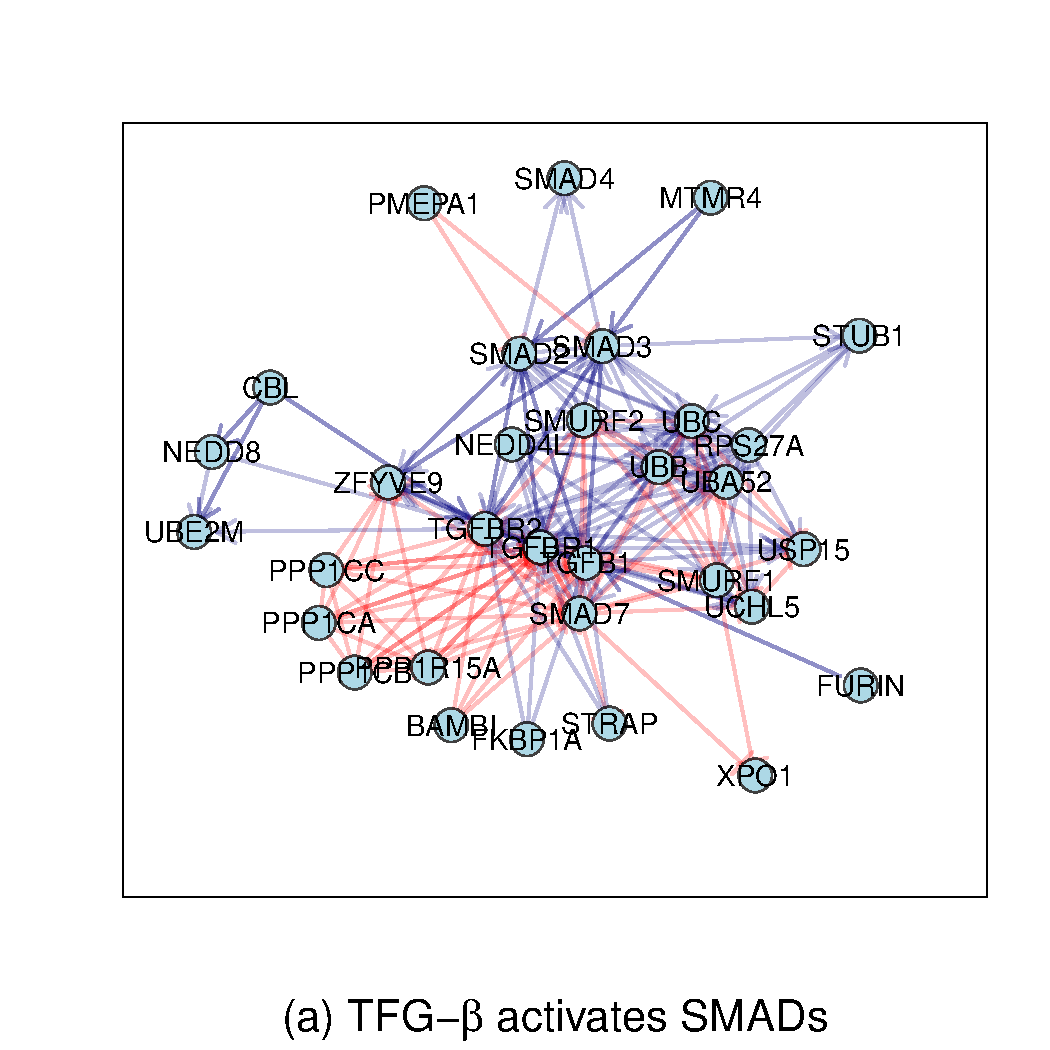
\includegraphics[width=.415\linewidth,height=.415\linewidth]{Plotsimulation_smad-1} 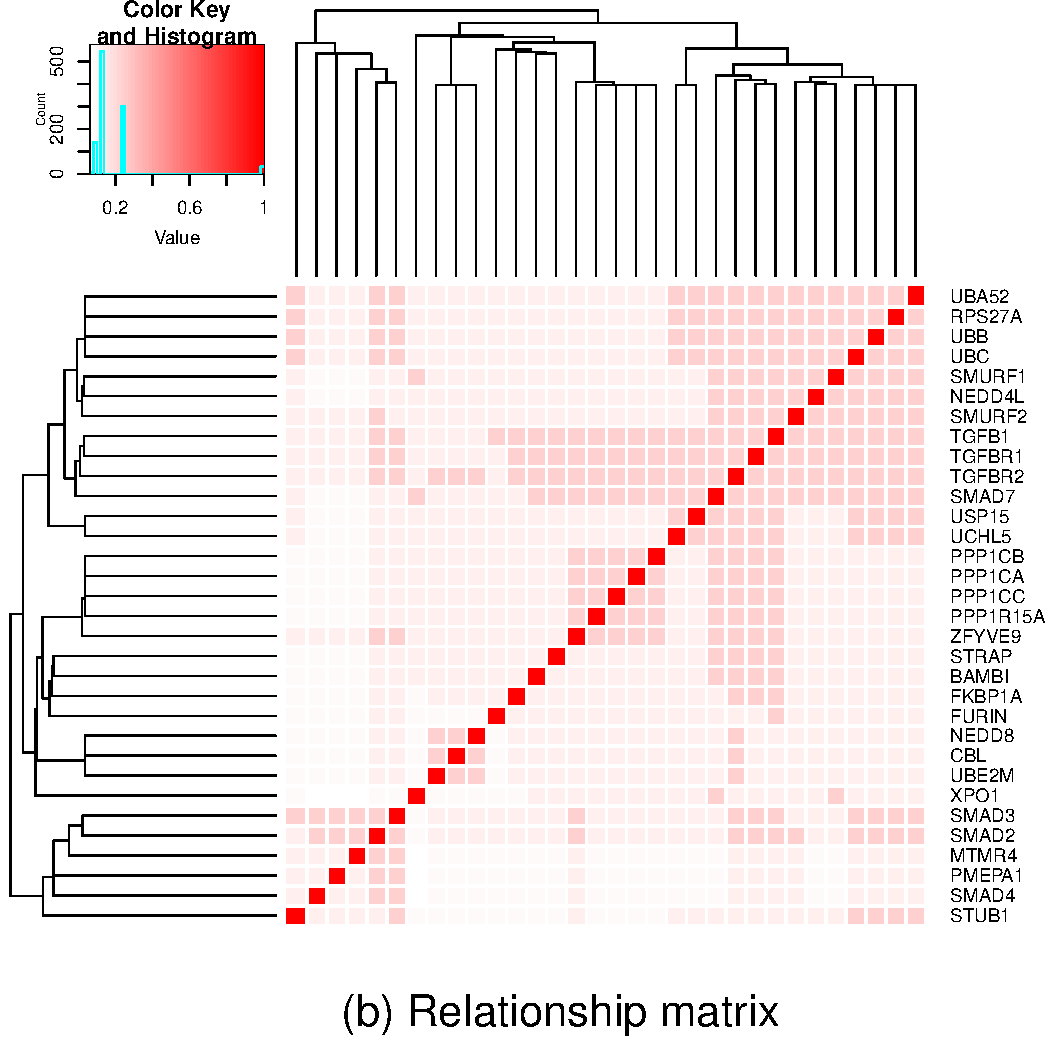
\includegraphics[width=.415\linewidth,height=.415\linewidth]{Plotsimulation_smad-2} 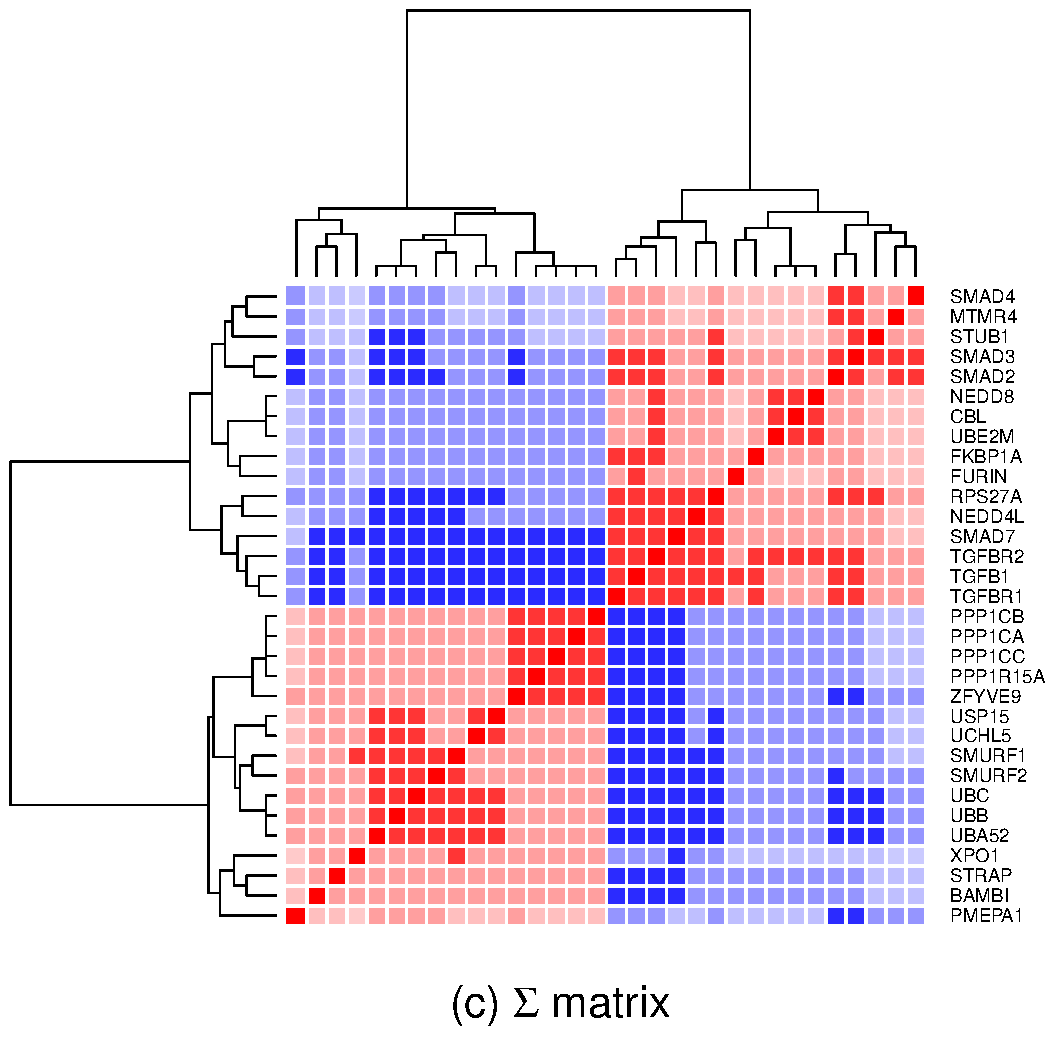
\includegraphics[width=.415\linewidth,height=.415\linewidth]{Plotsimulation_smad-3} 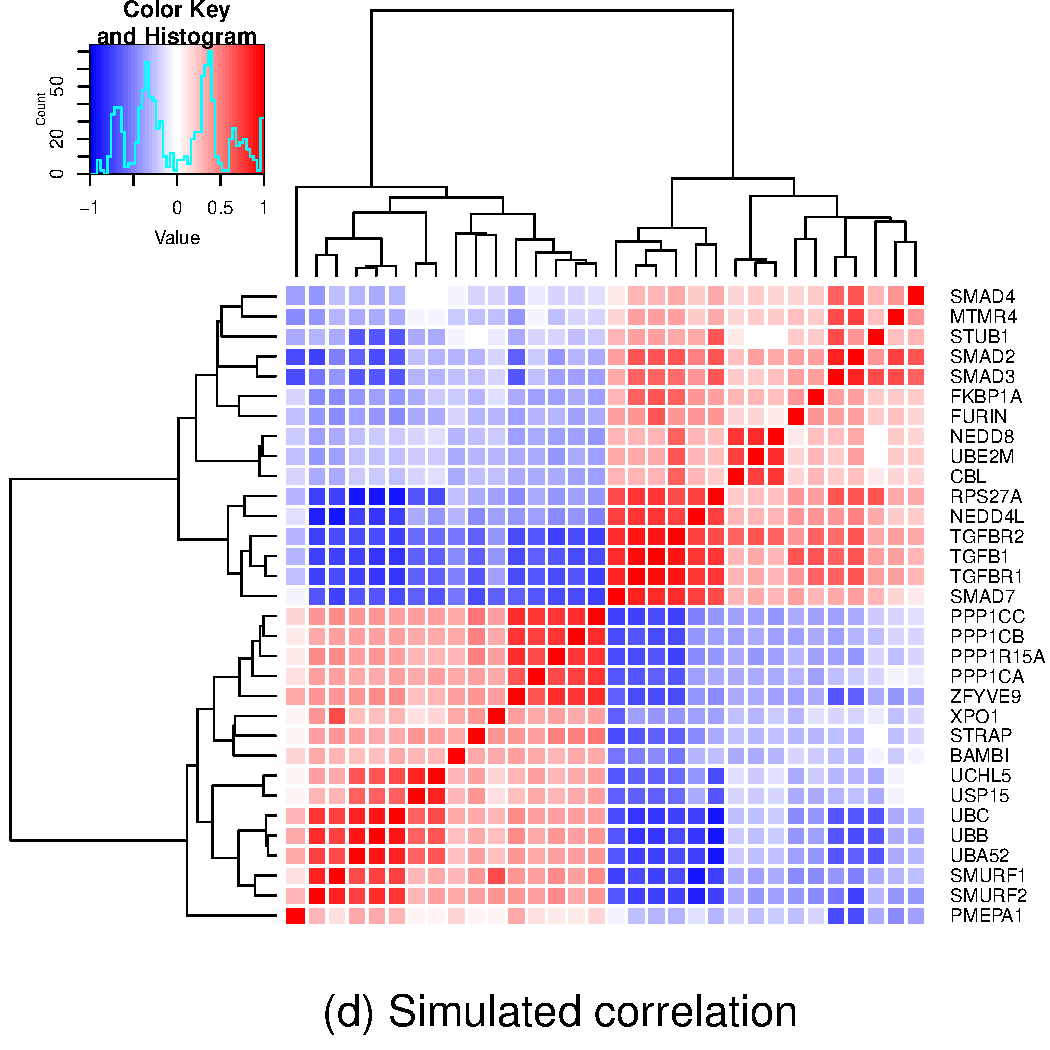
\includegraphics[width=.415\linewidth,height=.415\linewidth]{Plotsimulation_smad-4} 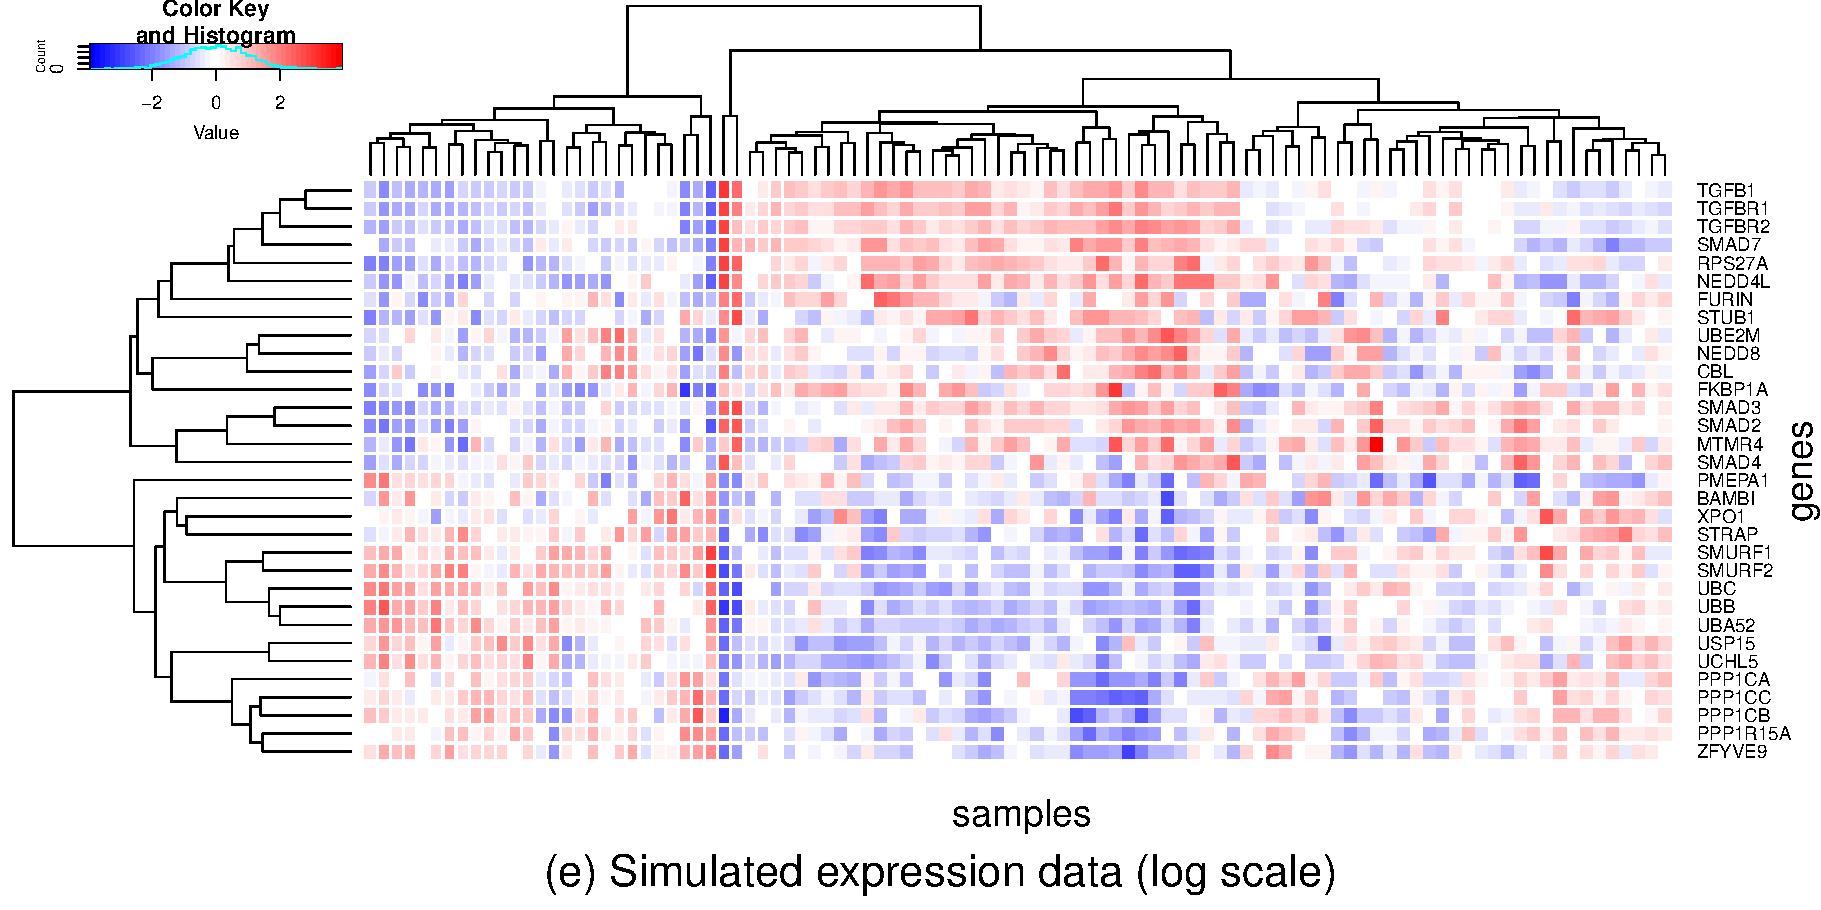
\includegraphics[width=.830\linewidth,height=.415\linewidth]{Plotsimulation_smad-5} 

}

\caption{\textbf{Simulating expression from a biological pathway graph structure}. The graph structure (a) of a known biological pathway, the TGF-$\beta$ receptor signaling activates SMADs (R-HSA-2173789), was used to derive a relationship matrix (b), $\Sigma$ matrix (c) and correlation structure (d) from the relative distances between the nodes. These values are coloured blue to red from $-1$ to $1$. This has been used to generate a simulated expression dataset of 100 samples (coloured blue to red from low to high) via sampling from the multivariate normal distribution. Here modules of genes with correlated expression can be clearly discerned.}\label{fig:simulation_smad}
\end{figure}

These simulated datasets can also be used for simulating gene expression
data within a graph network to test genomic analysis techniques.
Correlation structure can be included into datasets generated when
testing whether true positive genes or samples can be detected in a
sample with the background of complex pathway structure.

\hypertarget{sec:summary}{%
\section{Summary and discussion}\label{sec:summary}}

Biological pathways are of fundamental importance to understanding
molecular biology. In order to translate findings from genomics studies
into real-world applications such as improved healthcare, the roles of
genes must be studied in the context of molecular pathways. Here we
present a statistical framework to simulate gene expression from
biological pathways, and provide the \texttt{graphsim} package in R to
generate these simulated datasets. This approach is versatile and can be
fine-tuned for modelling existing biological pathways or for testing
whether constructed pathways can be detected by other means. In
particular, methods to infer biological pathways and gene regulatory
networks from gene expression data can be tested on simulated datasets
using this framework. The package also enables simulation of complex
gene expression datasets to test how these pathways impact on
statistical analysis of gene expression data using existing methods or
novel statistical methods being developed for gene expression data
analysis.

\hypertarget{computational-details}{%
\section*{Computational details}\label{computational-details}}
\addcontentsline{toc}{section}{Computational details}

The results in this paper were obtained using R 3.6.1 with the
\texttt{igraph} 1.2.4.1 \texttt{Matrix} 1.2-17, \texttt{matrixcalc}
1.0-3, and \texttt{mvtnorm} 1.0-11 packages. R itself and all dependent
packages used are available from the Comprehensive Archive Network
(CRAN) at \url{https://CRAN.R-project.org}. The \texttt{graphsim}
package presented can be installed from CRAN and the issues can be
reported to the development version on GitHub
(\url{https://github.com/TomKellyGenetics/graphsim}). This package is
included in the library on GitHub
(\url{https://github.com/TomKellyGenetics/igraph.extensions}) which
installs various tools for \texttt{igraph} analysis. This software is
cross-platform and compatible with installations on Windows, Mac, and
Linux operating systems. The package GitHub repository also contains
vignettes with more information and examples on running functions
released in the package. The package (\texttt{graphsim} 0.1.2) has been
released on CRAN and will be updated.

\hypertarget{acknowledgements}{%
\section*{Acknowledgements}\label{acknowledgements}}
\addcontentsline{toc}{section}{Acknowledgements}

This package was developed as part of a PhD research project funded by
the Postgraduate Tassell Scholarship in Cancer Research Scholarship
awarded to STK. We thank members of the Laboratory of Professor Satoru
Miyano at the University of Tokyo, Institute for Medical Science,
Professor Seiya Imoto, Associate Professor Rui Yamaguchi, and Dr Paul
Sheridan (Assistant Professor at Hirosaki University,CSO at Tupac Bio)
for helpful discussions in this field. We also thank Professor Parry
Guilford at the University of Otago, Professor Cristin Print at the
University of Auckland, and Dr Erik Arner at the RIKEN Center for
Integrative Medical Sciences for their excellent advice during this
project.

\hypertarget{contributions}{%
\section*{Author Contributions}\label{contributions}}
\addcontentsline{toc}{section}{Author Contributions}

S.T.K. and M.A.B. conceived of the presented methodology. S.T.K.
developed the theory and performed the computations. M.A.B. provided
guidance throughout the project and gave feedback on the package. All
authors discussed the package and contributed to the final manuscript.

\hypertarget{references}{%
\section*{References}\label{references}}
\addcontentsline{toc}{section}{References}

\hypertarget{refs}{}
\leavevmode\hypertarget{ref-Arner2015}{}%
Arner, E., C. O. Daub, K. Vitting-Seerup, R. Andersson, B. Lilje, F.
Drabløs, A. Lennartsson, et al. 2015. ``Transcribed enhancers lead waves
of coordinated transcription in transitioning mammalian cells.''
\emph{Science} 347 (6225): 1010--4.

\leavevmode\hypertarget{ref-Barabasi2004}{}%
Barabási, A. L., and Z. N. Oltvai. 2004. ``Network Biology:
Understanding the Cell's Functional Organization.'' \emph{Nat Rev Genet}
5 (2): 101--13.

\leavevmode\hypertarget{ref-Matrix}{}%
Bates, Douglas, and Martin Maechler. 2016. \emph{Matrix: Sparse and
Dense Matrix Classes and Methods}.
\url{https://CRAN.R-project.org/package=Matrix}.

\leavevmode\hypertarget{ref-Reactome}{}%
Croft, D, A F Mundo, R Haw, M Milacic, J Weiser, G Wu, M Caudy, et al.
2014. ``The Reactome pathway knowledgebase.'' Journal Article.
\emph{Nucleic Acids Res} 42 (database issue): D472--D477.
\url{https://doi.org/10.1093/nar/gkt1102}.

\leavevmode\hypertarget{ref-igraph}{}%
Csardi, Gabor, and Tamas Nepusz. 2006. ``The Igraph Software Package for
Complex Network Research.'' \emph{InterJournal} Complex Systems: 1695.
\url{http://igraph.org}.

\leavevmode\hypertarget{ref-Genz2009}{}%
Genz, Alan, and Frank Bretz. 2009. ``Computation of Multivariate Normal
and t Probabilities.'' In \emph{Lecture Notes in Statistics}. Vol. 195.
Heidelberg: Springer-Verlag.

\leavevmode\hypertarget{ref-mvtnorm}{}%
Genz, Alan, Frank Bretz, Tetsuhisa Miwa, Xuefei Mi, Friedrich Leisch,
Fabian Scheipl, and Torsten Hothorn. 2016. \emph{Mvtnorm: Multivariate
Normal and T Distributions}.
\url{http://CRAN.R-project.org/package=mvtnorm}.

\leavevmode\hypertarget{ref-Hawe2019}{}%
Hawe, J. S., F. J. Theis, and M. Heinig. 2019. ``Inferring Interaction
Networks From Multi-Omics Data.'' \emph{Front Genet} 10: 535.

\leavevmode\hypertarget{ref-Higham2002}{}%
Higham, N. J. 2002. ``Computing the Nearest Correlation Matrix--a
Problem from Finance.'' \emph{IMA Journal of Numerical Analysis} 22 (3).
Oxford University Press: 329--43.
\url{https://doi.org/10.1093/imanum/22.3.329}.

\leavevmode\hypertarget{ref-Hirose2008}{}%
Hirose, Osamu, Ryo Yoshida, Seiya Imoto, Rui Yamaguchi, Tomoyuki
Higuchi, D. Stephen Charnock-Jones, Cristin Print, and Satoru Miyano.
2008. ``Statistical Inference of Transcriptional Module-Based Gene
Networks from Time Course Gene Expression Profiles by Using State Space
Models.'' \emph{Bioinformatics} 24 (7): 932--42.
\url{https://doi.org/10.1093/bioinformatics/btm639}.

\leavevmode\hypertarget{ref-Hu2016}{}%
Hu, J. X., C. E. Thomas, and S. Brunak. 2016. ``Network biology concepts
in complex disease comorbidities.'' \emph{Nat. Rev. Genet.} 17 (10):
615--29.

\leavevmode\hypertarget{ref-Komatsu2013}{}%
Komatsu, M., T. Yoshimaru, T. Matsuo, K. Kiyotani, Y. Miyoshi, T.
Tanahashi, K. Rokutan, et al. 2013. ``Molecular features of triple
negative breast cancer cells by genome-wide gene expression profiling
analysis.'' \emph{Int. J. Oncol.} 42 (2): 478--506.

\leavevmode\hypertarget{ref-Law2014}{}%
Law, C. W., Y. Chen, W. Shi, and G. K. Smyth. 2014. ``voom: Precision
weights unlock linear model analysis tools for RNA-seq read counts.''
\emph{Genome Biol.} 15 (2). Springer Nature: R29.
\url{https://doi.org/10.1186/gb-2014-15-2-r29}.

\leavevmode\hypertarget{ref-Li2015}{}%
Li, P., Y. Piao, H. S. Shon, and K. H. Ryu. 2015. ``Comparing the
normalization methods for the differential analysis of Illumina
high-throughput RNA-Seq data.'' \emph{BMC Bioinformatics} 16 (October):
347.

\leavevmode\hypertarget{ref-Markowetz2007}{}%
Markowetz, F., and R. Spang. 2007. ``Inferring cellular networks--a
review.'' \emph{BMC Bioinformatics} 8 Suppl 6 (September): S5.

\leavevmode\hypertarget{ref-Ozsolak2011}{}%
Ozsolak, F., and P. M. Milos. 2011. ``RNA sequencing: advances,
challenges and opportunities.'' \emph{Nat. Rev. Genet.} 12 (2): 87--98.

\leavevmode\hypertarget{ref-Perou2000}{}%
Perou, C. M., T. Sørlie, M. B. Eisen, M. van de Rijn, S. S. Jeffrey, C.
A. Rees, J. R. Pollack, et al. 2000. ``Molecular portraits of human
breast tumours.'' \emph{Nature} 406 (6797): 747--52.

\leavevmode\hypertarget{ref-limma}{}%
Ritchie, Matthew E, Belinda Phipson, Di Wu, Yifang Hu, Charity W Law,
Wei Shi, and Gordon K Smyth. 2015. ``limma Powers Differential
Expression Analyses for RNA-Sequencing and Microarray Studies.''
\emph{Nucleic Acids Research} 43 (7): e47.

\leavevmode\hypertarget{ref-Shimamura2009}{}%
Shimamura, Teppei, Seiya Imoto, Rui Yamaguchi, André Fujita, Masao
Nagasaki, and Satoru Miyano. 2009. ``Recursive Regularization for
Inferring Gene Networks from Time-Course Gene Expression Profiles.''
\emph{BMC Systems Biology} 3 (1): 41.
\url{https://doi.org/10.1186/1752-0509-3-41}.

\leavevmode\hypertarget{ref-Svensson2018}{}%
Svensson, V., R. Vento-Tormo, and S. A. Teichmann. 2018. ``Exponential
scaling of single-cell RNA-seq in the past decade.'' \emph{Nat Protoc}
13 (4): 599--604.

\leavevmode\hypertarget{ref-Wang2018}{}%
Wang, J., M. Huang, E. Torre, H. Dueck, S. Shaffer, J. Murray, A. Raj,
M. Li, and N. R. Zhang. 2018. ``Gene expression distribution
deconvolution in single-cell RNA sequencing.'' \emph{Proc. Natl. Acad.
Sci. U.S.A.} 115 (28): E6437--E6446.

\leavevmode\hypertarget{ref-Yamaguchi2007}{}%
Yamaguchi, Rui, Ryo Yoshida, Seiya Imoto, Tomoyuki Higuchi, and Satoru
Miyano. 2007. ``Finding module-based gene networks with state-space
models - Mining high-dimensional and short time-course gene expression
data.'' \emph{IEEE Signal Processing Magazine} 24 (1): 37--46.

\end{document}
